% Created 2020-07-03 Fri 13:14
% Intended LaTeX compiler: pdflatex
\documentclass[10pt, a4paper]{article}
\usepackage[utf8]{inputenc}
\usepackage[T1]{fontenc}
\usepackage{graphicx}
\usepackage{grffile}
\usepackage{longtable}
\usepackage{wrapfig}
\usepackage{rotating}
\usepackage[normalem]{ulem}
\usepackage{amsmath}
\usepackage{textcomp}
\usepackage{amssymb}
\usepackage{capt-of}
\usepackage{hyperref}
\usepackage{titlesec}
\setcounter{secnumdepth}{4}
\titleformat{\paragraph}
{\normalfont\normalsize\bfseries}{\theparagraph}{1em}{}
\titlespacing*{\paragraph}
{0pt}{3.25ex plus 1ex minus .2ex}{1.5ex plus .2ex}
\usepackage[dvipsnames]{xcolor}
\usepackage{todonotes}
\usepackage{apacite}
\usepackage{lscape}
\usepackage[toc,page]{appendix}
\setlength{\parskip}{0.5em}
\hypersetup{colorlinks = true, linktocpage=true, filecolor = RoyalBlue, citecolor = RoyalBlue, linkcolor = RoyalBlue, urlcolor = RoyalBlue, unicode}
\setcounter{secnumdepth}{5}
\author{Njagi Mwaniki}
\date{\today}
\title{EXPLORING VIRUS SEQUENCE DIVERSITY USING GENOME GRAPHS}
\hypersetup{
 pdfauthor={Njagi Mwaniki},
 pdftitle={EXPLORING VIRUS SEQUENCE DIVERSITY USING GENOME GRAPHS},
 pdfkeywords={},
 pdfsubject={},
 pdfcreator={Emacs 26.3 (Org mode 9.2.4)}, 
 pdflang={English}}
\begin{document}

\begin{titlepage}
\centering
{\LARGE EXPLORING VIRUS SEQUENCE DIVERSITY USING GENOME GRAPHS \par }
\vspace {8cm}
{\small Njagi Mwaniki \par}
\vspace {8cm} 
{\small A thesis submitted in partial fulfilment of the             requirements for the award of a Master of Science Degree in             Bioinformatics of Pwani University. \par}
\vspace {1mm} 
{\small \today. \par}
\end{titlepage}
\urlstyle{same}
\newcommand{\bigO}{\mathcal{O}}

\pagenumbering{roman}

\setcounter{secnumdepth}{0}
\newpage

\section{Declaration}
\label{sec:org6914488}
This thesis is my original work and has not been presented for a degree in any other university or any other award.

\vspace{10mm}

Moses Njagi Mwaniki

Date …………………………    Signature …………………….…………

\vspace{20mm}
I confirm that the work reported in this thesis was carried out by the candidate under my supervision.

\vspace{10mm}

Dr George Githinji

Date …………………………    Signature …………………….…………

\vspace{10mm}

Dr Pjotr Prins

Date …………………………    Signature …………………….…………

\vspace{10mm}

Prof James Nokes

Date …………………………    Signature …………………….…………


\newpage

\section{Dedication}
\label{sec:org0752a2a}
I dedicate this project to \ldots{} for the strength and inspiration throughout the period and
to\ldots{}

\newpage
\section{Acknowledgement}
\label{sec:org8f67fa9}
I would like to express my deepest appreciation to\ldots{}.

\newpage
\pagewidth
\section{Abstract}
\label{sec:orgdc4d31d}
\begin{ABSTRACT}
Reference genomes represent a consensus assembly of the most frequent reads or
bases in a sample. Genome graphs use low level data structures to provide 
access to reads used in the assembly as a network of nodes where a node 
represents a sequence or kmer. In this work we used genome graphs to explore
and represent virus sequence diversity.

Respiratory Syncytial Virus samples were collected from a twenty-five-member 
household during a household outbreak and used to assemble a genome graph. 
Reads from each sample were mapped on to this graph and the number of reads that
mapped under each was noted. We then applied principal component analysis to 
reduce the 196,488-dimensional coverage data and the results used to generate 
distance matrices which were then summarised as a cladogram.

We established a method able to differentiate each of the samples by comparing
the depth of coverage of each sample against that of every other sample.
The use of different principle components, either the first principal component 
or the first five principal components, gave different topologies.
The first five provided a tree that was more parsimonious and closer to the
maximum likelihood tree generated in previous studies.

Our naïve approach provides an all vs all sample comparison of sample
relatedness using data provided by a genome graph. It also shows that sequence
coverage across a genome graph is an alternative approach to provide sequence 
relatedness.
\end{ABSTRACT}
\setcounter{secnumdepth}{4}

\newpage

\setcounter{tocdepth}{5}
\tableofcontents

\newpage
\listoffigures

\newpage
\pagenumbering{arabic}

\section{Introduction}
\label{sec:org5c6e6e3}
\subsection{Background Information}
\label{sec:org610ca9c}

RSV was first isolated in Chimpanzees in 1956 and named Chimpanzee Coryza Agent
\cite{morrisRecoveryCytopathogenicAgent1956}. 
A year later, in 1957, it was isolated in children from
whom it had not been possible to isolate and renamed Respiratory Syncytial
Virus \cite{beemAssociationChimpanzeeCoryza1960,chanockRecoveryInfantsRespiratory1957,zlatevaGeneticVariabilityMolecular2005}.

During the first year of life, RSV is the most frequent cause of acute lower
respiratory tract infection bringing infants between one and six months of age
into the hospital with pneumonia, bronchitis
\cite{stottRespiratorySyncytialVirus1985,zlatevaMolecularEvolutionCirculation2004,borchersRespiratorySyncytialVirus2013}, 
and otitis \cite{kleinRoleRespiratorySyncytial1982} and significantly increases the prevalence of
asthma amongst children who are hospitalized with RSV in infancy or early
childhood \cite{borchersRespiratorySyncytialVirus2013}. Moreover, there is a marked correlation
between the incidence of RSV in the community and the occurrence of sudden
infant deaths in children above 3 months of age \cite{chanockRecoveryInfantsRespiratory1957}.
A simple upper respiratory illness in high-risk immunocompromised adults is no
longer viewed as trivial \cite{whimbeyRespiratorySyncytialVirus2000}. 
People with cardiopulmonary diseases and immunocompromised persons with bone
marrow transplant patients prior to marrow engraftment are at highest risk for
pneumonia and death \cite{morrisRecoveryCytopathogenicAgent1956}.
For cancer patients, the risks and benefits of
administering intensive chemotherapy in the setting of a seemingly benign upper
respiratory illness are now weighed heavily \cite{kleinRoleRespiratorySyncytial1982}.

In animals, the virus is recognized as an important cause of Bovine Respiratory
Disease (BRD) in Europe and the United States \cite{whimbeyRespiratorySyncytialVirus2000}.

In terms of its epidemiology, it produces an annual epidemic of predominantly 
upper respiratory tract infections in children and healthy adults
\cite{chanockRecoveryInfantsRespiratory1957} with re-infections occurring throughout
life even in the presence of pre-existing antibodies \cite{sullenderGeneticDiversityAttachment1991}.
\subsection{Problem Statement}
\label{sec:orgdc33092}
Conventional methods of describing diversity involve comparing each sample
against a given reference genome instead of comparing every sample against every
other sample \cite{patenGenomeGraphsEvolution2017}. This comparison is
non-transitive meaning that the way a sample varies from the reference does not
expressly tell us how that sample varies from a separate sample. 
\subsection{Justification}
\label{sec:orgce626ec}
A reference genome graph is a robust data structure for representing genome
variation unlike the current approach where we compare a sample against a
linear reference genome. Given that consensus sequences are a mosaic of
haplotypes, we would like to make use of genome graph to disentangle the
sequence diversity present in RSV sequences, and potentially other respiratory
viruses. 
\subsection{Objectives}
\label{sec:org531612f}
\subsubsection{Main Objective}
\label{sec:orga9fdbfa}
To construct an RSV variation graph from samples collected from a single
household in the course of an RSV household outbreak.
\subsubsection{Specific Objectives}
\label{sec:org94cf5b8}
\begin{enumerate}
\item To perform a review of existing genome graph tools used in constructing pangenome graphs.
\item To construct a variation graph from a set of samples collected from a single
household during the course of an RSV epidemic.
\end{enumerate}
\newpage
\section{Literature Review}
\label{sec:org0b18c1d}
\subsection{RNA Viruses}
\label{sec:org8fa4595}
RNA viral populations don’t exist as a collection of organisms with a single
genome but rather as a quasispecies
(also called a mutant spectrum or a mutant cloud) where most of the biologically
relevant variation observed in vivo is as a result of genetic variation,
competitive selection and random events acting on multiple replicative units.
These quasispecies dynamics have been used to explain the failure of
monotherapy and synthetic antiviral vaccines but have opened new possibilities
for antiviral interventions \cite{domingoViralQuasispeciesEvolution2012}.
These viruses have mutation rates up to a million times higher than their hosts;
rates that are so high it is unlikely for a virus to have an identical RNA
molecule as its immediate progeny \cite{domingoViralQuasispeciesEvolution2012}. 
Negative selection controls this mutation rate and proof that it is not 
optimized by natural selection is that in some cases it leads to local
extinction \cite{duffyWhyAreRNA2018}.

\subsubsection{Respiratory Syncytial Virus (RSV)}
\label{sec:orgdb492b2}
RSV is the major cause of acute lower respiratory tract infections associated 
with pneumonia, bronchitis (Borchers et al., 2013; Zlateva et al., 2004) and
otitis \cite{kleinRoleRespiratorySyncytial1982} more frequently than any other agent and
particularly in the first year of life \cite{stottRespiratorySyncytialVirus1985}.
As if that wasn’t enough, RSV significantly increases the prevalence of asthma
in children who are hospitalized with it and there is a marked correlation
between the incidence of RSV in the community and the occurrence of sudden
infant deaths as well as a third of cot deaths among children over 3 months of
age \cite{chanockRecoveryInfantsRespiratory1957}. 

A simple upper respiratory illness in immunocompromised adults or the elderly
is no longer viewed as trivial
\cite{chanockRecoveryInfantsRespiratory1957,whimbeyRespiratorySyncytialVirus2000}.
People with cardiopulmonary diseases and immunocompromised persons with bone
marrow transplant patients prior to marrow engraftment are at highest risk for
pneumonia and death \cite{morrisRecoveryCytopathogenicAgent1956}.
For cancer patients, the risks and
benefits of administering intensive chemotherapy in the setting of a seemingly
benign upper respiratory illness are now weighed heavily
\cite{kleinRoleRespiratorySyncytial1982}.

In animals, the RSV virus is also recognized as an important cause of Bovine
Respiratory Disease (BRD) in Europe and the United States
\cite{whimbeyRespiratorySyncytialVirus2000} being the most costly disease of beef
cattle in North America \cite{griffinEconomicImpactAssociated1997}.

\paragraph{History}
\label{sec:org39999af}
The virus was first isolated in 1956 from Chimpanzees and named Chimpanzee
Coryza Agent \cite{morrisRecoveryCytopathogenicAgent1956} after which it was
isolated in children from whom it had not been possible to isolate and renamed 
RSV in 1957 then classified in order Mononegavirales, family Paramyxoviridae,
subfamily Pneumovirinae, genus Pneumovirus
\cite{chanockRecoveryInfantsRespiratory1957,beemAssociationChimpanzeeCoryza1960,zlatevaGeneticVariabilityMolecular2005}.

\paragraph{Epidemiology}
\label{sec:org3fa1d66}
In older children and healthy adults, RSV presents in highly seasonal annual
epidemics (Aamir et al., 2013; Al-Toum et al., 2006) of mild reinfections
predominantly in the upper respiratory tract (Chanock et al., 1957) even in the
presence of pre-existing antibodies (Cane, 2001; Sullender et al., 1991).

The epidemics have been found to have a significant negative correlation with
temperature and a significant positive correlation with relative humidity and
rainfall \cite{al-toumEpidemiologyClinicalCharacteristics2006}
and therefore crop up in the coldest months which naturally vary with latitude.

In temperate climates, RSV epidemics occur in the winter between December and
February but peaking in January and February  (Al-Toum et al., 2006) and are a
major cause of winter mortality associated with 60-80\% more deaths than
influenza \cite{nicholsonImpactInfluenzaRespiratory1996}.

In tropical climates, epidemics occur during the rainy season
\cite{al-toumEpidemiologyClinicalCharacteristics2006,aamirMolecularCharacterizationCirculating2013} 
but are also associated with religious festivals
\cite{caneMolecularEpidemiologyRespiratory2001}.

Serious disease is limited to the primary infection which occurs between six
weeks and two years of age during the child’s first or second epidemics
\cite{caneMolecularEpidemiologyRespiratory2001} and can occur in the presence of
maternally derived antibodies.
However, infants with more severe illnesses were found to have lower levels of
antibodies in serum collected near the onset of illness than did infants with
milder illnesses 
\cite{glezenRiskRespiratorySyncytial1981,caneMolecularEpidemiologyRespiratory2001}.

\paragraph{The Genetic Makeup of RSV}
\label{sec:org11d6928}
\begin{figure*}[h!]
\centering
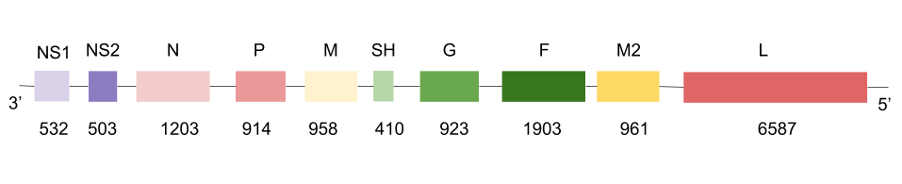
\includegraphics[width=0.75\textwidth]{figures/RSV-genes.png}
\caption[RSV Antisense RNA Strand]{\label{fig:orgf223893}
A schematic of RSV antisense RNA strand showing its 10 genes. The rectangles represent genes with the different shades of the same colour used to show similarity. The grey connectors are the intergenic regions. The numbers below are the estimated gene lengths. Adapted from \cite{namRespiratorySyncytialVirus2019}.}
\end{figure*}

\begin{figure*}[h!]
\centering
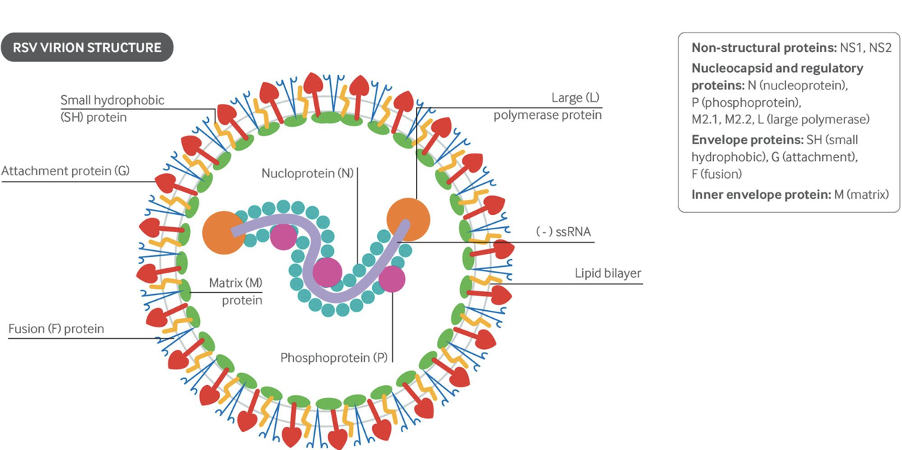
\includegraphics[width=0.75\textwidth]{figures/RSV-cross-section.png}
\caption[RSV Capsid]{\label{fig:orgb6c2945}
A schematic of the RSV capsid showing the lipid bilayer and most importantly the surface the F and G glycoproteins. From \cite{namRespiratorySyncytialVirus2019}.}
\end{figure*}

RSV, whose genome structure is shown above, is an enveloped virus with a
nonsegmented negative-strand RNA genome of approximately 15,200 nucleotides
containing 10 genes which code for 11 proteins whose order is 3k NS1, NS2, N,
P, M1, SH, G, F, M2 (note that M2 codes for M2.1 and M2.2 proteins), and L with
attenuation of transcription step-wise with distance from the 3k end
\cite{caneMolecularEpidemiologyRespiratory2001}.

As shown in table 1 and figures 1 and 2, RSV has three surface glycoproteins:
the small hydrophobic (SH) protein which may be non-structural, the fusion (F)
protein which plays the main role in virus penetration, syncytium formation,
and possibly can also mediate attachment and the attachment (G) glycoprotein
which plays the main role in virus attachment. It has four nucleocapsid
proteins including the nucleoprotein (N), phosphoprotein (P),
M2-1(also designated 22K and sometimes considered a matrix protein) and
polymerase (L). 
The M2 gene contains a second open reading frame encoding a protein (M2-2) which
regulates transcription (Fearns \& Collins, 1999). There is a single matrix 
protein, M1, which may mediate interactions between the nucleocapsid and
envelope and the two non-structural proteins, NS1 and NS2  have recently been 
shown to antagonise the interferon-induced antiviral response
\cite{fearnsRoleM21Transcription1999,schlenderBovineRespiratorySyncytial2000}.
\paragraph{Groups of RSV}
\label{sec:org44d29d5}
RSV was initially divided into two antigenic groups A and B in 1966 by its 
reaction with panels of monoclonal antibodies particularly those directed
against its P, F and G proteins \cite{coatesAntigenicAnalysisRespiratory1966}. 
It is worth noting that only antibodies directed against the G and F proteins
have been shown to be neutralising in vitro or protective in vivo
\cite{caneMolecularEpidemiologyRespiratory2001}. 

It was later demonstrated that the two groups are distinct at the genetic level
\cite{johnsonFusionGlycoproteinsHuman1988}.
The F and N proteins are highly conserved
between the groups showing 91\% and 96\% amino acid similarity, respectively 
\cite{johnsonFusionGlycoproteinsHuman1988,johnson1BNS21C1989}.
In contrast, the G protein was found to be highly variable where the amino acid
similarity of this protein between groups A and B was 53\%
\cite{johnsonGlycoproteinHumanRespiratory1987,zlatevaMolecularEvolutionCirculation2004}.

Both groups are known to circulate within an epidemic \cite{peretCirculationPatternsGenetically1998}
without any leading to the extinction of the other, although A tends to be more
dominant in epidemics attributed to the higher variability among the A strains
\cite{peretCirculationPatternsGenetically1998,zlatevaGeneticVariabilityMolecular2005}.

The sequence diversity of the G glycoprotein (the type II glycoprotein of
289–299 amino acids depending on the virus strain
\cite{caneMolecularEpidemiologyRespiratory2001}  coded by the 
G gene suggests that the two subgroups have evolved separately for a significant
period of time with proof of RSV A’s most recent common ancestor dating back as
the early 1940s \cite{zlatevaMolecularEvolutionCirculation2004}.

Because the F gene mutates at a much lower rate compared to the G gene it
becomes an adequate vaccine target which is why we talk of RSV F vaccines 
\cite{andersonStrategicPrioritiesRespiratory2013,giersingReportWorldHealth2016}. 
This lower rate of mutation also leads to consistent identification by
antibodies and therefore the major neutralizing antibody response to RSV appears
to be induced by the F protein \cite{olmstedExpressionGlycoproteinRespiratory1986}.

Groups A and B are subdivided further into subgroups, as of 2012 there were 11
subgroups of RSV A: ON1, GA1–GA7, SAA1, NA1, and NA2 and 17 subgroups of RSV
B: GB1–GB4, SAB1-SAB3, and BA1–BA10
\cite{peretCirculationPatternsGenetically1998,peretCirculationPatternsGroup2000,venterGeneticDiversityMolecular2001,trentoMajorChangesProtein2003,shobugawaEmergingGenotypesHuman2009,eshaghiGeneticVariabilityHuman2012,aamirMolecularCharacterizationCirculating2013}.

\newpage

\subsection{Graphs in Bioinformatics}
\label{sec:orgd7b01be}
Contemporary methods of representing a reference genome as a linear sequence of 
characters to represent bases \cite{diltheyImprovedGenomeInference2015} introduce a
mapping bias towards alleles in the reference known as reference bias compared
to the mapping of alternative alleles
\cite{degnerEffectReadmappingBiases2009,brandtMappingBiasOverestimates2015}. 

This naturally leads to a need for a structure that can represent variation that
is inherent in the genome. Other models can approach this structure with
varying degrees of accuracy, but it is naturally represented as a graph in
which the sequences themselves are implicitly encoded as walks in the graph
\cite{patenGenomeGraphsEvolution2017}.
\newpage

\subsection{Graph Theory}
\label{sec:org515a8bf}
A graph is an object, or collection, of two sets, a vertex set and edge set.
The vertex set is a finite non-empty set, to mean a graph must have at least one
vertex.
The edge set may be empty \cite{trudeauIntroductionGraphTheory1993}
and is used to present relationships between the vertices.

More formally, a graph G is an unordered pair (V(G), E(G)) consisting of a set
V(G) of vertices and a set E(G), disjoint from V (G), of edges, together with
an incidence function that associates with each edge of G an unordered pair of
(not necessarily distinct) vertices of G \cite{bondyGraphTheory2011}.

Graphs can be represented diagrammatically as shown in Figure \ref{fig:org5ea1eb6}.

G \{\{a c\} \{b d\}\}
H \{\{a c\} \{c d\}\}
\begin{figure*}
\centering
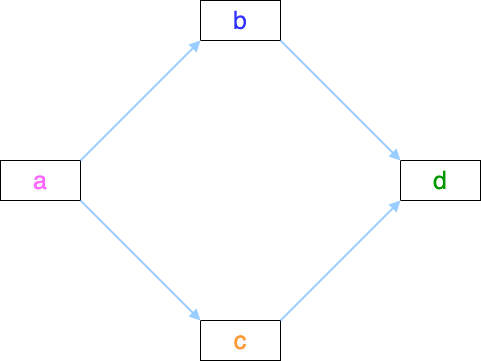
\includegraphics[width=0.7\textwidth]{figures/Graph-classifications-Digraph.png}
\caption[Generic Graph Example]{\label{fig:org5ea1eb6}
}
\end{figure*}
\begin{figure*}
\centering
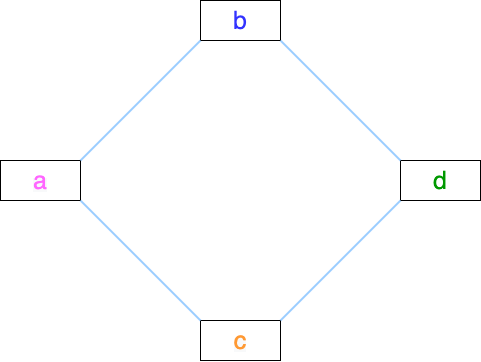
\includegraphics[width=0.7\textwidth]{figures/Graph-classifications-Undirected.png}
\caption[Generic Graph Example]{\label{fig:org5ea1eb6}
}
\end{figure*}

\subsubsection{Graph classifications}
\label{sec:org58ab2ac}
Graphs can be broken down into many classifications but in this case, we want to
focus on simple versus multigraphs and directed versus undirected.
A simple graph can only have one edge connecting two adjacent vertices while a
multigraph is a graph in which two adjacent vertices are connected by more than
one edge.

Simple Graph
\begin{figure*}
\centering

\includegraphics[width=0.7\textwidth]{figures/Graph-classifications-Simple-Graph.png}
\caption[Simple Graph]{\label{fig:org4e7087d}
A simple graph showing only a single edge connecting any two nodes}
\end{figure*}


Multigraph
\#+CAPTION [Multigraph]: A multigraph where more than one edge can connect any two nodes.
\begin{figure*}
\centering
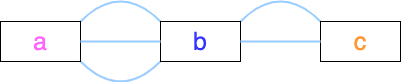
\includegraphics[width=0.7\textwidth]{figures/Graph-classifications-Multigraph.png}
\label{org61c4b03}
\end{figure*}


Figure 3: (a) A simple graph showing only a single edge connecting any two
nodes. (b) A multigraph where more than one edge can connect any two nodes.
A directed graph also called a digraph is a graph in which the edges have
direction.

Figure 4: A directed graph with the edges indicating direction.
An undirected graph is one in which the edges do not have direction indicated on
them.

Figure 5: An undirected graph where the edges have no indication of direction.
A bidirected graph is one in which each edge has an independent orientation
\cite{edmondsMatchingWellSolvedClass2003}.
This is important for the representation of strand, that is reading a DNA
molecule in its forward or reverse complement orientation 
\cite{patenGenomeGraphsEvolution2017}.

The degree of a vertex v in a graph G, is the number of edges of G incident with
v (going in and out of v), each loop counting as two edges. In directed graphs,
we have the concept of indegree and outdegree. The indegree refers to the
numbers of head ends of the edges adjacent to a vertex and the outdegree is the
number of tail ends of the edges adjacent to a vertex \cite{bondyGraphTheory2011}.
A vertex is even if its degree is an even number and odd otherwise
\cite{trudeauIntroductionGraphTheory1993}.

An isomorphism, in \ref{fig:orgd1e16b1}, is a relationship between two graphs such that the two graphs
can be represented by identical diagrams \cite{bondyGraphTheory2011} whereas an 
automorphism of a graph is an isomorphism of the graph to itself as shown below.

\begin{figure*}
\centering
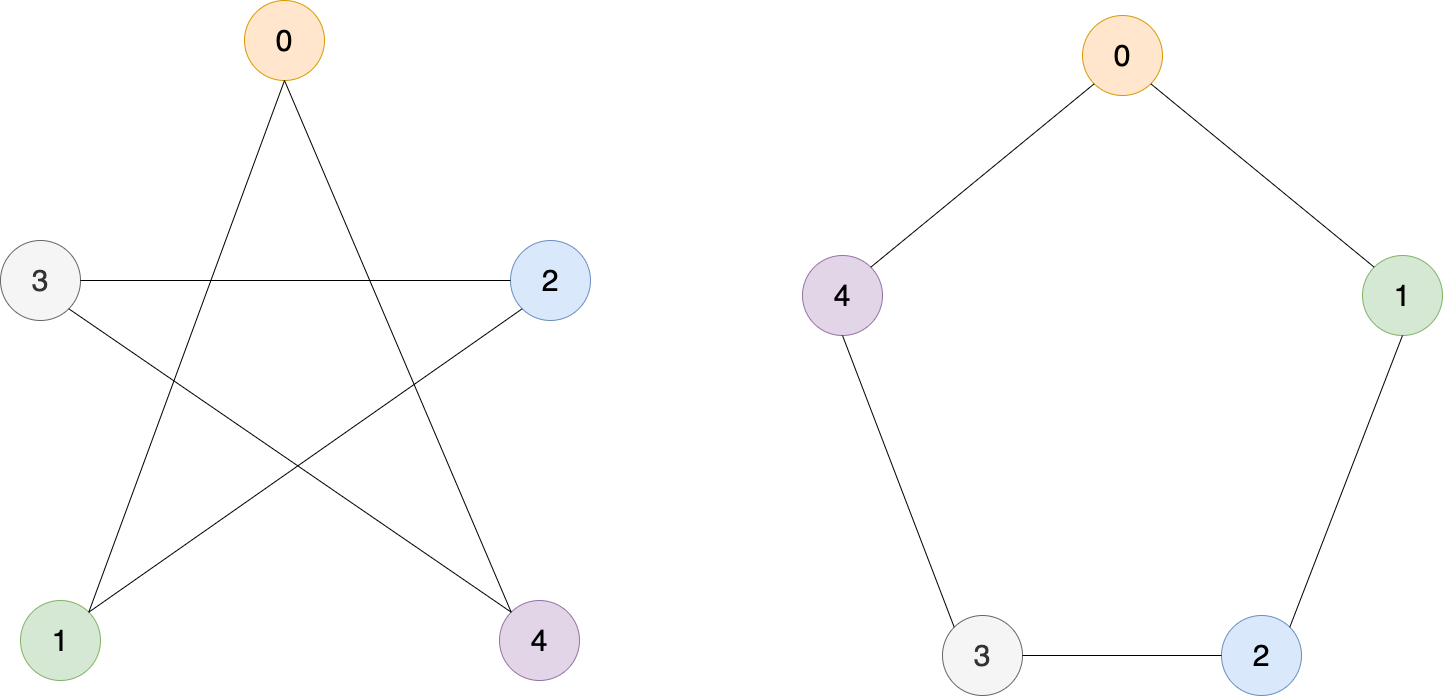
\includegraphics[width=0.7\textwidth]{figures/Isomorphism.png}
\caption[Isomorphism]{\label{fig:orgd1e16b1}
The two nodes are different visualizations of the same graph and therefore an isomorphism.}
\end{figure*}

\subsubsection{Walks and paths}
\label{sec:org9541cbd}
A path is a simple graph whose vertices can be arranged in a linear sequence in
such a way that two vertices are adjacent if they are consecutive in the 
sequence, and are nonadjacent otherwise \cite{bondyGraphTheory2011}.

A walk in a graph is a sequence A1 A2 A3 \ldots{} An of not necessarily distinct 
vertices in which A1 is joined by an edge to A2, A2 is joined by an edge to
A3, \ldots{}, and An−1 is joined by an edge to An. The walk A1 A2 A3 \ldots{} An is said
to join A1 and An \cite{trudeauIntroductionGraphTheory1993}.

Therefore, a path is a graph, whereas a walk is a traversal of a graph.

An Euler or Eulerian walk is a walk that uses every edge in the graph exactly
once.

A Hamiltonian walk is like an eulerian walk but for nodes and can be open or
closed, an open hamilton walk is a walk that uses every vertex in the graph
exactly once. A closed hamilton walk is a closed walk that uses the initial
vertex exactly twice and all the other vertices in the graph exactly once
\cite{trudeauIntroductionGraphTheory1993}.

\newpage

\subsection{Genome Graphs}
\label{sec:orge2ca0dd}
A genome graph is a generic term that refers to the representation of a sequence
or sequences or genetic material using graph-based methods implicitly or
explicitly. Genome graphs are expected to lead to improvements in mapping reads,
variant calling and haplotype determination \cite{patenGenomeGraphsEvolution2017}.

Genome graphs are generally directed graphs and have different classifications,
based on where the sequences are held within the graph, either on the edge or in
the nodes.

These are vertex-labelled directed graphs, graphs whose nodes are labelled such
that a directed walk can be interpreted as a DNA sequence, defined by the
sequence of node labels along the walk and edge-labelled directed graphs in
which case the nodes, rather than the edges, can be viewed as representing the 
intersection points between connected subsequences
\cite{patenGenomeGraphsEvolution2017}.

\subsubsection{De Bruijn Graph}
\label{sec:org26a4fc9}
These are graphs used in the assembly of reads named after Dutch mathematician
Nicolaas de Bruijn who became interested in the superstring problem: find a 
shortest circular superstring that contains all possible substrings of length k
(k-mers) over a given alphabet which he solved using an eulerian walk over the
k-mers \cite{compeauHowApplyBruijn2011}.

\subsubsection{Sequence graph}
\label{sec:org2a05df6}
A sequence graph is a bidirected graph in which each node is labelled with a
nucleotide string a “sequence graph” \cite{patenGenomeGraphsEvolution2017}.
In this bidirected graph, the features of an edge indicate to which side of a 
node (sequence), 5’ or 3’, each end of the edge connects" \cite{novakGenomeGraphs2017}.

\subsubsection{Variation Graph}
\label{sec:org3531430}
A variation graph is a graph where a complete walk along the graph represents a
haplotype \cite{patenGenomeGraphsEvolution2017}.

Many genome graphs don’t represent the concept of the strand, "reading a DNA
molecule in its forward and reverse complement orientations". To express
strandedness, directed graphs can be generalized to bidirected graphs
\cite{edmondsMatchingWellSolvedClass2003,medvedevComputationalMethodsDiscovering2009}
in which each edge endpoint has an independent orientation, indicating whether 
the forward or the reverse complement strand of the attached node is to be
visited when entering the node through that endpoint of the edge.
Inversions, reverse tandem duplications, and arbitrarily complex rearrangements
are expressible in the bidirected representation
\cite{patenGenomeGraphsEvolution2017}.

\subsubsection{Population Reference Graphs (PRGs)}
\label{sec:org928237e}
Population reference graphs are graphs that represent a population-wide genome
combining multiple reference sequences and catalogues of variation
\cite{diltheyImprovedGenomeInference2015}. 
This concept may also be extended to represent, in our case, a virus mutant
cloud.

\subsubsection{Problems arising from graph-based reference models}
\label{sec:orgc73f1e4}
\paragraph{Calling alleles at sites}
\label{sec:orgae9429c}
This involves declaring an allele at a given position, this position could span
several nodes or edges in an undefined manner. 

A proposed way to describe their positions is via motif
\cite{patenGenomeGraphsEvolution2017}, patterns of interconnections occurring
in complex networks at numbers that are significantly higher than those in
randomized networks \cite{miloNetworkMotifsSimple2002}, called a superbubble in directed graph
or an ultrabubble in bidirected graphs \cite{patenSuperbubblesUltrabubblesCacti2017}.

Superbubbles and ultrabubbles are directed acyclic subgraphs that connect to the
rest of the graph through one source node and one sink node
\cite{patenSuperbubblesUltrabubblesCacti2017}.
\paragraph{Non-trivial indexing and reference mapping}
\label{sec:org31a9824}
We now need to use methods that are aware of alternative alleles to map reads to
a graph reference \cite{patenGenomeGraphsEvolution2017}. 
The indexing could be done through gbwt \cite{sirenHaplotypeawareGraphIndexes2018}
could be achieved via partial order alignment gssw \cite{zhaoSSWLibrarySIMD2013}.
\paragraph{Coordinate system}
\label{sec:org870a87f}
A reference genome coordinate system is a system that uses coordinates to
uniquely determine the positions of bases in the reference genome 
\cite{randCoordinatesIntervalsGraphbased2017}.

An interesting problem introduced by graph-based reference structures is that
it’s no longer trivial to define a locus on the reference
\cite{patenGenomeGraphsEvolution2017}. The Computational Pan-Genomics
Consortium (2016) however agreed on qualities that a coordinate system should 
have \cite{patenGenomeGraphsEvolution2017,randCoordinatesIntervalsGraphbased2017}.
A coordinate system should have: monotonicity genome graph coordinates of
successive bases within a genome should be increasing, legibility coordinates 
should be compact and human interpretable, spatiality bases physically close
together within a genome should have similar coordinates, vertical spatiality
of bases that are allelic variants of one another
\cite{randCoordinatesIntervalsGraphbased2017}. 
horizontal spatiality of bases that can appear together within a single molecule
\cite{randCoordinatesIntervalsGraphbased2017}.
\subsubsection{Mapping reads to a reference genome graph}
\label{sec:org3b9fb94}
Given that a genetic sequence is read in small pieces for short reads and much
longer pieces for long reads, we need to find where in the genome a read comes
from. Read mapping is the process of finding the position where the read came
from in a reference sequence or graph \cite{novakGenomeGraphs2017}.
\paragraph{Reference bias or reference allele bias}
\label{sec:org4fed999}
Reference allele bias is the tendency to under-report data whose underlying DNA
does not match a reference allele \cite{patenGenomeGraphsEvolution2017}.
Masking known SNP positions in the genome sequence can eliminate the reference
bias but do not lead to more reliable results overall
\cite{degnerEffectReadmappingBiases2009}.

\subsubsection{Variation Graphs in Virus Haplotype Detection and Quantification}
\label{sec:orge40d267}
Compared to eukaryotes, viruses have relatively short genomes and high mutation 
rates \cite{duffyWhyAreRNA2018} and RNA viruses exist as a quasi-species 
\cite{domingoViralQuasispeciesEvolution2012}. This gives rise to the need to
deconvolute the individual haplotypes and quantify them.

There are a number of other tools for the assembly of haplotypes of virus
quasispecies.
These can be broadly categorized into reference-guided and reference-free.
De novo approaches do not require any prior information, such as a reference
genome or knowledge of the quasispecies composition. De novo approaches have
been shown to have advantages over reference-guided reconstruction, since using
a reference genome can induce significant biases
\cite{baaijensStrainawareAssemblyGenomes2020}.

There exist methods for de novo, strain aware metagenomic assembly such as 
VG-flow \cite{baaijensStrainawareAssemblyGenomes2020} however which focus only on 
short-read data.
VG-flow takes as input a next-generation sequencing (NGS) data set and a 
collection of strain-specific contigs assembled from the data and produces 
full-length haplotypes and corresponding abundance estimates 
\cite{baaijensStrainawareAssemblyGenomes2020}.
\subsection{A Review of Genome Graph Tools}
\label{sec:org0e0e444}
\subsubsection{Fragment Assembly}
\label{sec:org218e364}
The fragment assembly problem, reconstructing long contigs from reads
\cite{chikhiCompactingBruijnGraphs2016}, started with Sanger sequencing.
Like solving a puzzle of sequences the assembly problem can be framed as finding
a set of common super-strings from a set of substrings to which tools take
either a Eulerian, connect the nodes, or a Hamiltonian, connect the edges,
approach.

\paragraph{Overlap Graph}
\label{sec:org0b59421}
The first solution was SEQAID, short for \textbf{seq}uencing \textbf{aid},
\cite{peltolaSEQAIDDNASequence1984} which used the  Overlap Layout Consensus (OLC)
framework, an intuitionistic approach to the assembly problem that works in
3 main steps: 1) Overlap: find all overlaps among the reads, 2) Layout: assemble
a graph of all the reads based on their overlaps, and 3) Consensus: infer the
consensus sequence.

It finds the overlaps between the given set of reads and then lays
them out to form a DAG. The graph, however, has multiple paths that are the
genome or superstring in question. Which is where the consensus comes in.
It used … to infer the consensus.

\begin{figure*}[h]
\centering
\includegraphics[width=0.7\textwidth]{../Figures/OLC_Framework.png}
\caption[Overlap Graph]{\label{fig:org0f25d23}
OLC\ldots{}}
\end{figure*}

With the advent of Second-Generation Sequencing (SGS) technologies:
Roche/454 (\url{http://www. 454.com}), Illumina/solexa (\url{https://www.illumina.com}),
and AB/Solid (\url{https://www.thermofisher.com}) there was a significant reduction in
the cost per sequenced nucleotide \cite{liComparisonTwoMajor2012} leading to an
explosion in the number of reads produced and thus making OLC unfeasible.

\paragraph{de Bruijn Graph}
\label{sec:org29caef5}
OLC based methods were progressively replaced by de Bruijn Graph (DBG)
\cite{iduryNewAlgorithmDNA1995} based methods whose first tool was EULER
\cite{pevznerEulerianPathApproach2001}.

The DBG transforms the assembly problem into a computationally simpler problem.
While the OLC, through the reads graph, takes an non polynomial time Hamiltonian
approach; the DBG, using the k-mer graph, goes about it using a much easier to
solve Eulerian approach which works in polynomial time.
\cite{liComparisonTwoMajor2012,pevznerEulerianPathApproach2001}

The DBG is an anti-intuitionistic solution whose assembly quality improves with
an increase in the read length <citation needed>. It works through 1) chop the reads into
much smaller k-mers, 2) Use all the k-mers to assemble a dBG, 3) Infer the
genome sequence on the dBG. These tools made it possible to work with the
increasing number of reads produced.

\begin{figure*}[h]
\centering
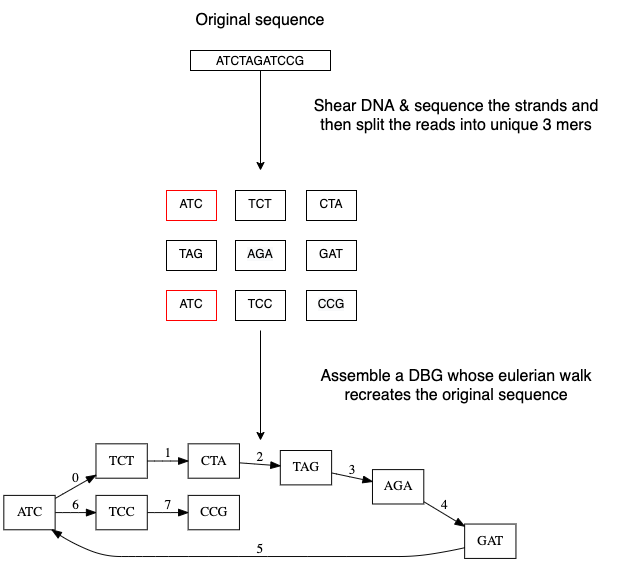
\includegraphics[width=0.7\textwidth]{../Figures/de Bruijn Graph.png}
\caption[de Bruijn Graph]{\label{fig:orgeb2a687}
DBG \ldots{}}
\end{figure*}

Lately, Single Molecule Sequencing (long read sequencing)  methods have
reintroduced OLC for the assembly of long erroneous reads but DBG based methods
are still used to correct long reads.
The unitig approach involves finding the maximal interval subgraphs in the
graph of all read overlaps.

\paragraph{String Graph}
\label{sec:org06fdc88}
The string graph \cite{myersFragmentAssemblyString2005} is a way to infer the
genome from the read data without a need for k-mers as is with the de Bruijn
graph.  It treats the genome as a sequence of repeats and then encodes each
repeat as a node. Each unique (contiguous) sequence is a node.
An Eulerian tour recreates the genome.

\begin{figure*}[h]
\centering
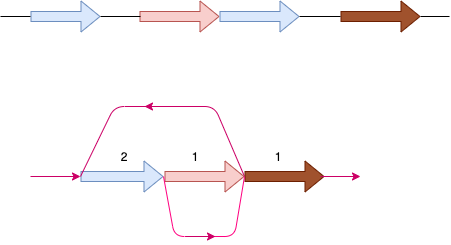
\includegraphics[width=0.7\textwidth]{../Figures/String Graph.png}
\caption[String Graph]{\label{fig:org9716fbd}
String Graph \ldots{}}
\end{figure*}

\subsubsection{Alignment and mapping}
\label{sec:orgc00f6c7}
Alignment involves computing the amount of similarity between two strings also
known as the edit distance problem.
The solution to the edit distance problem by
\cite{levenshteinBinaryCodesCapable1966a} paved the way for solving the alignment
problem.

The first solution was global alignment
\cite{needlemanGeneralMethodApplicable1970} in which a sequence query is aligned
to the other (reference) in its entirety. It took a dynamic programming approach
which worked in square time (had a complexity of \(\bigO(n^2)\); it was followed
by semi-global alignment \cite{sellersTheoryComputationEvolutionary1980}
where one sequence (query) is entirely
aligned to a substring of the other (reference); then local alignment
\cite{smithIdentificationCommonMolecular1981}, where the alignment can be between
any substrings of the two sequences.

In practice when given a set of reads, a complement of each read is generated to
be searched against because of the direction of sequencing or inversions.
A match can either be exact, matching the pattern exactly, or fuzzy, where a
section or all of the string matches the pattern approximately, with minimum
edit distance.

With graphs, reads are mapped to paths in the graph instead of linear sequences.
Alignment problems grow with the input size
\cite{durbinEfficientHaplotypeMatching2014} making it hard to align sequences to
graphs  because of the increased amount of data involved
The complexity of an alignment problem is a function of the
number of  vertices |V| and edges |E| <citation needed>.  In some way you can
think of it as mapping to multiple linear sequences that may or may not loop.

\subsubsection{Indexing}
\label{sec:org0038561}
Indexing is a solution to the problem of search given limited computing
resources. In bioinformatics we may want to find (also called mapping) where, 
if at all, a sequence occurs in a reference genome or graph.

An index makes mapping and alignment feasible within given time and memory
requirements by reducing the search space therefore reducing the time taken and
memory consumed when performing a search. \todo{cite this}

\paragraph{Search and index classifications}
\label{sec:orgfc86610}
Indexes can be classified based on how they are stored or how they are built.

\subparagraph{Static vs dynamic indexes}
\label{sec:orgd89aa0e}
A static index is serialized and saved to disk while a dynamic index is created
at runtime and held in memory. 

Dynamic indices are good with small datasets that change rapidly such as in the
construction of a DBG making it suitable for fragment assembly. Static indices
are suited for larger datasets that we want to go back to such as a reference
genome graph.\todo{cite}

\subparagraph{On-line vs off-line search algorithms}
\label{sec:org41a71ee}
When searching through reference genomes the reference changes at a much lower
rate than the queries and we also want to optimize the computational cost of
searching through our text. 
Whether one chooses to optimize or not is dependent on the problem but in the
case of alignment and mapping it is clear that optimization is the better
option.
Algorithms that perform this optimization are said to be offline while those
that don't optimize are said to be on-line while algorithms that don't are
off-line \cite{borodinOnlineComputationCompetitive1998}.

\paragraph{Optimization methods}
\label{sec:org7edd0bb}
There are many different ways of optimizing the search space for indexing.
In this case I only cover the ones relevant to the \hyperref[sec:orgdfdf803]{index implementations}
covered.

\subparagraph{Burrows-Wheeler Transform}
\label{sec:orgc673c2f}
Introduced by \cite{burrowsBlocksortingLosslessData1994}, the Burrows-Wheeler
Transform (BWT) is a reversible permutation of a string built by
lexicographically ordering all the permutations of a string then extracting its
last column. A faster way to generate a BWT is through a \hyperref[sec:orgb4d02d0]{Suffix Array}.

As shown in figure \ref{fig:run length encoding}, the BWT of a string or in this
case a nucleotide sequence
has a property that like characters cluster together in runs which allows for
compression.
In fact, the BWT was originally built for text compression and to this day
forms the basis of the bzip2 (\url{https://sourceware.org/bzip2/}) compression algorithm.

\begin{figure*}[h]
\centering
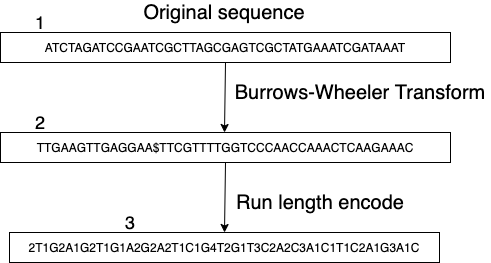
\includegraphics[width=0.7\textwidth]{../Figures/Run Length Encoding.png}
\caption[Run Length Encoding Using a Burrows Wheeler Transform]{\label{fig:org34b8bd7}
The BWT of a string showing like characters clustering together in runs and being compressed through run length encoding.}
\end{figure*}



The BWT on it's own isn't an index but it is a step in creation of compressible
indexes whose compressibility doesn't hinder performance such as the suffix
array or the FM index.

\subparagraph{Suffix Array}
\label{sec:orgb4d02d0}
Suffix arrays, introduced by \cite{manberSuffixArraysNew1990}, are arrays of the
positions of all the sorted suffixes of a string.
A suffix array is a simple, space efficient
(stores n integers where n is the length of the string) alternative to the
suffix tree.

An improvement to the suffix array by \cite{liMinimapMiniasmFast2016} provided
the first in-place \(\bigO(n)\) time suffix array construction algorithm that
is optimal both in time and space, where in-place means that the algorithm only
needs \(\bigO(1)\) additional space beyond the input string and the output suffix
array.

Tools using the suffix array include Bowtie
\cite{langmeadUltrafastMemoryefficientAlignment2009}, BWA
\cite{liFastAccurateShort2009},
and SOAP2 \cite{liSOAP2ImprovedUltrafast2009}.

\paragraph{Index implementations}
\label{sec:orgdfdf803}
\subparagraph{FM Index}
\label{sec:orgf775ac7}
Short for Full-text index in Minute space, the FM index
\cite{ferraginaOpportunisticDataStructures2000} is a full text substring index
based on the BWT. It allows compression of the input text while permitting fast
substring queries. It can be used to efficiently find the number of occurrences
of a pattern within the compressed text, as well as locate the position of each
occurrence.

\subparagraph{Positional Burrows-Wheeler Transform}
\label{sec:orgbf6d7a3}
Introduced by \cite{durbinEfficientHaplotypeMatching2014} Positional Burrows
Wheeler Transform is an algorithm with complexity \(\bigO(NM)\) where M sequences
and N bi-allelic sites.
It derives a representation of the data based on a positional prefix array; an
array that holds positions of a given array/set of haplotypes in a larger
haplotype array. This prefix array orders them in reverse (ascending) order of
their prefixes allowing similar sequences to cluster together.

<Add PBWT table and graphic>

\subparagraph{GBWT/gPBWT}
\label{sec:orgb94f1f1}
First described \cite{novakGraphExtensionPositional2017} but used in a tool
\cite{sirenHaplotypeawareGraphIndexes2020} it’s a compressible representation of
a set of haplotypes held in the graph. This allows for efficient match queries
in sections of the haplotypes (local alignment). Because of the previously
mentioned nature of the positional suffix array to bring together (fairly)
similar haplotypes.
GBWT lets us have an efficient way of counting the number of haplotypes
containing a given sequence.

\subparagraph{Bloom filters}
\label{sec:orga785802}
The bloom filter is a probabilistic data structure that can give false positive
but never a false negative. It works by hashing data and stores the hash in an
array.
Bloom filters can be used as the underlying implementation of a de Bruijn Graph 
because of its constant time access \cite{chikhiSpaceefficientExactBruijn2013}. 
It however suffers from poor data localization \todo{expound} which led to the
use of Blocked Bloom Filters (BBF) \cite{putzeCacheHashSpaceefficient2010} used in
Bifrost \cite{holleyBifrostHighlyParallel2019}.

\subparagraph{Minimizers}
\label{sec:orgbefd713}
Minimizers reduce the search space by generating k-mers from a read and sorting
them alphabetically. The k-mer at the top is the minimizer for that read\ldots{} 
then binning the result.
When a query is made it’s prefix is checked against the bin and the rest of the
data ignored <is this even accurate?>
We can get a minimizer by BBF blocked bloom filter Minimizers
\cite{grabowskiDiskbasedCompressionData2015,robertsReducingStorageRequirements2004}.
\todo{improve this section}
\subparagraph{Hash tables}
\label{sec:orgb1ef199}
Hash tables involve breaking down the reads into k-mers and storing the kmers
into hash tables that point to the original data. When queries are made they’re
similarly broken down into k-mers of the expected size<citation needed>.
Hash based methods when well tuned can be faster than suffix array based
methods, because the basic operations are simpler, but they typically require
greater memory, particularly in cases where the suffix representation can be
compressed as it can be here (Durbin 2014).
Many times tools take a hybrid approach; incorporating different aspects of
different indexing schemes such as in Minimap
\cite{liDesignConstructionReference2020}. \todo{ensure this citation checks out}

\paragraph{Indexes on linear references}
\label{sec:orgeca80f4}
In linear references commonly used indexing approaches are the FM index
\todo{list tools} whose complexity is \(\bigO(NM)\) where there are N variable
sites and M sequences \cite{durbinEfficientHaplotypeMatching2014}.
As in alignment, the problem grows even larger with the proliferation of paths
in graphs. For graphs, indices like the FM-index backed by the BWT fail to hold
<citation needed> and there’s the need for improvements such as that seen in
gBWT used in seqwish allowing it to be orders of magnitude faster than VG.

\paragraph{Indexes on graphs}
\label{sec:org1eb51bf}
Graph indexing started with GenomeMapper,
\cite{schneebergerSimultaneousAlignmentShort2009}, which demonstrated that
mapping short reads to a graph allowed access to polymorphisms that were
otherwise inaccessible through linear references.
It used a hash-based static index that was persisted to disk implemented as a 
mapping of k-mers to their positions in the graph. For performance, it converted
the k-mers unambiguously into integers by applying a 2-bit representation of
each nucleotide, and to avoid loading duplicate k-mers into memory it used
memory mapping to allow different processors access to the same piece of data.
GCSA, short for Generalized Compressed Suffix Array,
\cite{sirenIndexingGraphsPath2014} is a generalization of the Burrows Wheeler
Transform based FM index to graphs. 
Later, the variation graph toolkit used GCSA2
\cite{sirenIndexingVariationGraphs2017} whose index was based on de Bruijn graphs.

\subsubsection{Genome Graph Tools}
\label{sec:org322320d}
There are a lot of tools that apply the previously mentioned principles but
because the number tools is large and constantly growing I cover the subset that
I found useful for my applications with viruses.
\paragraph{Fragment Assembly}
\label{sec:orga182797}
\cite{myersFragmentAssemblyString2005} introduced the Berkeley Open Assembler
which borrowed from the unitig algorithm and used the \hyperref[sec:org06fdc88]{string graph},
a fragment assembly method that infers the genome from the read data without a
need for k-mers.
It treats the genome as a sequence of repeats and then encodes each repeat as
a node. Each unique (contiguous) sequence is a node. An Eularian tour recreates
the genome.

Though the original DBG approach does much better than OLC it still has a high
memory footprint <citation needed> therefore minia
\cite{chikhiSpaceefficientExactBruijn2013} proposed the encoding of a
de Bruijn Graph as a bloom filter (BF). It is obtained by inserting all the
nodes of a de Bruijn graph (i.e all k-mers) in a bloom filter instead of
storing the graph in a “traditional” set series of nodes and edges stored in a
more conventional graph structure such as an adjacency list.
A BF has a search/access time of  \(\bigO(1)\) and can give a false positive
result but never a false negative therefore the name probabilistic de Bruijn
graph.
They therefore had an additional structure to remove critical false positives.
It showed that the graph can be encoded with as little as 4 bits per node.
Drawbacks of using the bloom filter include 1) The Bloom filter introduces false
nodes and false branching, 2) The global structure of the graph is approximately
preserved up to a certain false positive rate.

Bcalm2 \cite{chikhiCompactingBruijnGraphs2016} tried to improve the BF backed dBG
by use of a compacted DBG (cdBG) which allowed the problem to be doable on a PC.

\todo{add compaction diagram}

The use of the de Bruijn graph in fragment assembly consists of a multi-step
pipeline.
The most data intensive steps are usually the first three: 1) nodes
enumeration/k-mer counting: the set of distinct k-mers is extracted from the
reads 2) Compaction: all unitigs (paths with all but the first vertex having
in-degree 1 and all but the last vertex having out-degree 1) are compacted into
a single vertex 3) graph cleaning: artifacts due to sequencing errors and
polymorphism are removed from the graph.

\cite{liMinimapMiniasmFast2016} introduced two tools minimap, a raw read
overlapper, and miniasm \cite{liMinimapMiniasmFast2016}, an assembler.
Minimap uses minimizer sketches, stores k-mers in a hash table, uses sorting
extensively.

BAUM (By Adaptive Unique Mapping) \cite{wangBAUMImprovingGenome2018} improved on
the OLC framework to improve genome assembly based on Second Generation Sequencing
paired-end/mate-pair libraries.
BAUM has two modules: 1) construction of the genome unique regions that are taken
as the initial contigs iterative assembly, in which scaffolds are built, and 2)
contigs are extended and merged, aiming to reconstruct the repetitive regions
along the iterations.
In this scheme, the repetitive regions are separated by the unique regions.

Bifrost \cite{holleyBifrostHighlyParallel2019} improved on the compacted de Bruijn
Graph by adding colours to the nodes to keep track of the source of each vertex
and takes advantage of concurrency (parallell).
A disadvantage of colors is that their size can grow beyond that of the
nodes/actual graph. It stores these colours in a different on a different
.bfg\textsubscript{colors} file.
K-mers contained in the unitigs are mapped to their colors representing the
input sources (color is represented by an integer from 1 to |C| where C is the
number of colors. Colors are stored in a separate array of color containers,
each color container is indexed by MPHF (Minimal Perfect Hash Function) library
BBHash \cite{limassetFastScalableMinimal2017}.
Bloom filters have have poor data localization because one element is scattered
all over which leads to CPU cache misses when inserting and querying are
addressed here  (Putze et al., n.d.) for this they used (BBF) blocked bloom filter
Minimizers \cite{robertsReducingStorageRequirements2004,grabowskiDiskbasedCompressionData2015}.
BBF works by building an approximation of the dBG using BBFs to filter our
sequencing errors.  BBF containing k-mers is used to build the cdBG.

\paragraph{Mapping and Alignment}
\label{sec:orgcc7603b}
GraphAlighner \cite{rautiainenBitparallelSequencetographAlignment2019} is a tool
for aligning long error prone reads to genome graphs through base alignment.
It uses (generalizes two linear sequence-to-sequence algorithms to graphs) two
strategies: 1) the Shift-And algorithm for exact matching (exact match of a
substring to a string) and 2) Myer’s bit-vector algorithm for semi-global
alignment. It Aligns sequences to graphs while exploiting bit parallelism.
Makes use of Nondeterministic Finite Automaton (NFA).
Store an NFA state bitvector for each node and update until no more change is
necessary Myer’s bit-vector algorithm studies the semi-global sequence-to-graph
alignment problem.
It seeks to find a path in a directed, node-labelled graph that has the
minimum edit distance to the query sequence. Myers’ bit-vector alignment
algorithm \cite{myersFastBitvectorAlgorithm1999} to graphs, which proceeds along
the same lines as the Shift-And algorithm, but requires some further algorithmic
insights to handle nodes with an in-degree greater than one.
Bitvector algo complexity grows approximately linearly with the number of
vertices in the graph.
The bitvector it uses is the size of the pattern we are searching for.
Semi-global alignment is solved through generalizing DP edit distance problem
for graphs.
Semi-global alignment is used to align a shorter seq against a longer one,
reference.
Shift-And algorithms (Baeza-Yates and Gonnet, 1992; Domolki, 1964, 1968)
performs exact string matching to graphs.
Their aim is to find a path in a directed, node-labeled graph that has a minimum
edit distance \cite{levenshteinBinaryCodesCapable1966a} to the query sequence.
Shift-And algo finds exact matches between a pattern string and a text string by
simulating a nondeterministic finite automaton (NFA) that matches the pattern
and then feeding the text to it.
Keep shifting the bit-vector by one and bitwise AND-ing the state.
Somewhat analogous to exact matching using a window of the size of the pattern.
It can handle DAGs and  graphs that may contain cycles. For DAGs, process the
nodes in topological order (topological sort). For cyclic graphs no sorting.

Minigraph \cite{liDesignConstructionReference2020} is a sequence to graph mapper
that incrementally constructs a pangenome graph.
A graph-based data model and associated formats to represent multiple genomes
while preserving the coordinate of the linear reference genome.
A straightforward way to represent a pangenome store unaligned genomes in a
full-text index that compresses redundancies in sequences identical between
individuals
\cite{makinenStorageRetrievalHighly2010,liuDeBWTParallelConstruction2016,boucherPrefixfreeParsingBuilding2019}.
The other class of methods encodes multiple genomes into a sequence graph,
usually by collapsing identical or similar sequences between genomes onto a
single representative sequence. The results in a pangenome graph.

\paragraph{End to End tools}
\label{sec:org0199189}

SPAdes also a toolkit does…

\paragraph{Graphical Analysis}
\label{sec:orgd8a61df}
Variation graphs are genome graphs that embed the paths in the graph
(citation needed).
These paths can be used to represent haplotypes. vg, HashGraph, odgi and
PackedGraph are dynamic (allow for updates to the graph while xg isn’t).

\definecolor{mypink}{RGB}{225, 0, 128}
\definecolor{mygreen}{RGB}{106, 168, 79}
\definecolor{myblue}{RGB}{111, 168, 220}
\definecolor{myred}{RGB}{225, 0, 0}
\definecolor{mypurple}{RGB}{153, 0, 255}

\begin{center}
\begin{tabular}{llllllll}
\color{mypink}Individual 1 & \color{mypink} A & \color{mypink} C & \color{mypink} T & \color{mypink} G & \color{mypink} A & \color{mypink} A & \color{mypink} T\\
\color{myblue}Individual 2 & \color{myblue} A & \color{myblue} C & \color{myblue} T & \color{myblue} T & \color{myblue} - & \color{myblue} - & \color{myblue} T\\
\color{mygreen}Individual 3 & \color{mygreen} A & \color{mygreen} C & \color{mygreen} T & \color{mygreen} T & \color{mygreen} A & \color{mygreen} A & \color{mygreen} T\\
\hline
\color{red}Consensus & \color{red} A & \color{red} C & \color{red} T & \color{red} T & \color{red} A & \color{myred} A & \color{red} T\\
\end{tabular}
\end{center}


\begin{figure*}[h!]
\centering
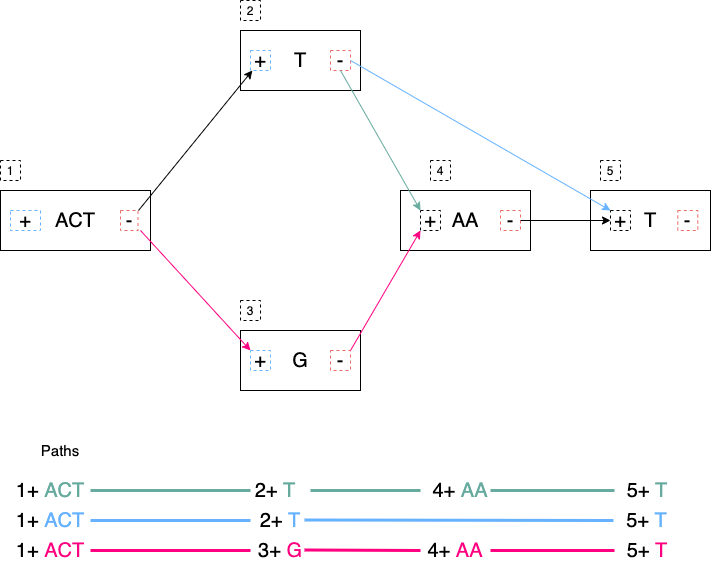
\includegraphics[width=0.7\textwidth]{../Review/figures/Variation Graph-Page-1.png}
\caption[Variation Graph]{\label{fig:orgb1ee106}
A variation graph with the paths outlined at the bottom}
\end{figure*}


In case of addition of individual 4 containing an inversion at node 2,3 and 4

\begin{center}
\begin{tabular}{llllllll}
\color{mypink}Individual 1 & \color{mypink} A & \color{mypink} C & \color{mypink} T & \color{mypink} G & \color{mypink} A & \color{mypink} A & \color{mypink} T\\
\color{myblue}Individual 2 & \color{myblue} A & \color{myblue} C & \color{myblue} T & \color{myblue} T & \color{myblue} - & \color{myblue} - & \color{myblue} T\\
\color{mygreen}Individual 3 & \color{mygreen} A & \color{mygreen} C & \color{mygreen} T & \color{mygreen} T & \color{mygreen} A & \color{mygreen} A & \color{mygreen} T\\
\color{mypurple}Individual 4 & \color{mypurple} A & \color{mypurple} C & \color{mypurple} A & \color{mypurple} A & \color{mypurple} T & \color{mypurple} T & \color{mypurple} T\\
\hline
\color{red}Consensus & \color{red} A & \color{red} C & \color{red} T & \color{red} T & \color{red} A & \color{myred} A & \color{red} T\\
\end{tabular}
\end{center}


\begin{figure*}[h!]
\centering
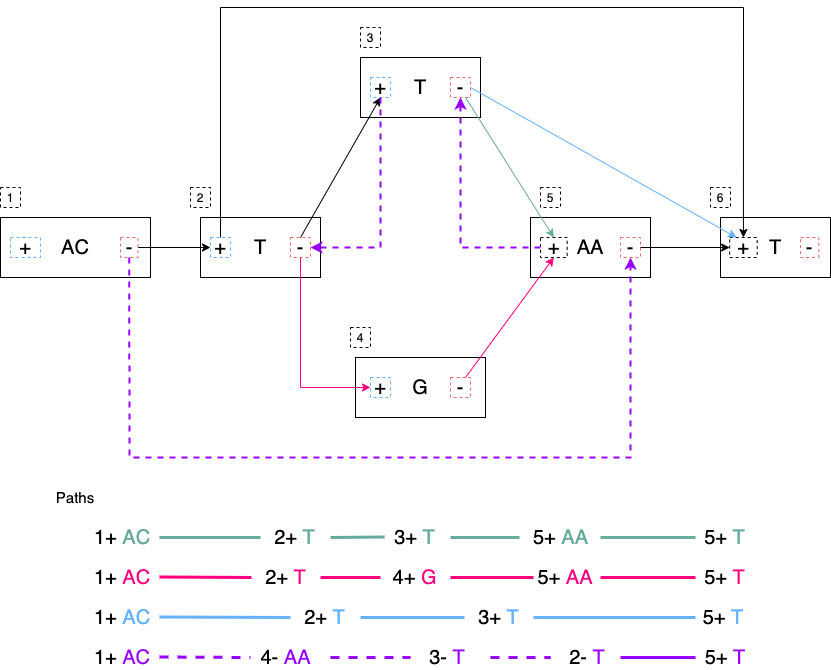
\includegraphics[width=0.7\textwidth]{../Review/figures/Variation Graph-Page-2.png}
\caption[Variation Graph with Inversion]{\label{fig:org8b413f7}
A variation graph represeting the paths but containing an inversion in individual 4}
\end{figure*}

vg \cite{garrisonVariationGraphToolkit2018} is an end to end pangenome graph
solution for de novo and incremental graph building but has large memory
requirements when it comes to indexing.
It originally used the protobuf library as the graph implementation but was
refactored to use the HandleGraph API as of 1.22.0.
The underlying graph holding nodes in a vector/linked and uses hash tables to
 map between nodes and ids in the vector that holds the nodes.
Paths are stored in a set of linked lists.
A hash table maps between nodes and paths and queries (of what) involve hash
table lookups.
Suffered from a problem of data duplication (citation needed).
It deals with cycles in the graph by unrolling the graph
\cite{liDesignConstructionReference2020}.

xg \cite{garrisonGraphicalPangenomics2019} is a memory-efficient succinct
representation of the graph (compared to vg).
It has fast queries thanks to a static index of the paths that is backed by
positional indices, GBWT.

Bluntification \cite{gargGraphbasedApproachDiploid2018} removing all overlaps
between nodes (is this not compaction?).

Seqwish (\url{https://github.com/ekg/seqwish}) transforms a set of
sequences and alignments (in GFA) into its equivalent variation graph.
The large memory requirements of vg are solved through the use of gBWT backed
by a Generalized Compressed Suffix Array.

HashGraph (libhandlegraph paper) has speed as its primary goal and achieves this
by representing the graph as a high performance hash table.
Paths are embedded as double linked lists.
Edges are in vectors attached to each node they connect.
Use an adjacency list which is appropriate for sparse graphs.
It is appropriate for small graphs (such as viruses) because it trades memory
for time.

It’s still a static index odgi (libhandlegraph paper)
Optimized Dynamic Graph Interface, uses a dynamic index and uses an in memory
variation graph to perform sorting, pruning, transformation, and visualization.
Odgi (libhandlegraph paper) is based on a node centric encoding of the graph that
is designed to improve cache coherency when traversing or modifying the graph.
It tries to be a pragmatic tool that achieves balance between memory usage and
performance. Each nodes seq and edges are encoded in a byte array using a
variable length integer, edges are described in terms of the relative offset of
a node in a sorted graph. PackedGraph (libhandlegraph paper) is designed to have
a low memory footprint.
It does this by encoding the graph mainly using linked lists.


vg-flow \cite{baaijensStrainawareAssemblyGenomes2020} attempts to reconstruct all
individual haplotypes from a mixed sample at the strain level and to provide
abundance estimates for the strains. It does this by\ldots{}

\subsubsection{Interfaces and APIs}
\label{sec:org46e3da7}
The field of genome graphs is growing quickly as evidenced by the ever-growing
number of tools creating the need for a common way for these tools interact with
the data they operate on.

One such solution is libhandlegraph \cite{eizengaSuccinctDynamicVariation2020}, a
declarative approach towards graphs that defines an interface between which
tools interact with the data below.
The idea is to treat the graph as a larger structure to which we have pointers,
called handles (similar to  Unix file handles), through which we manipulate the
graph.

\begin{figure}[h]
\centering
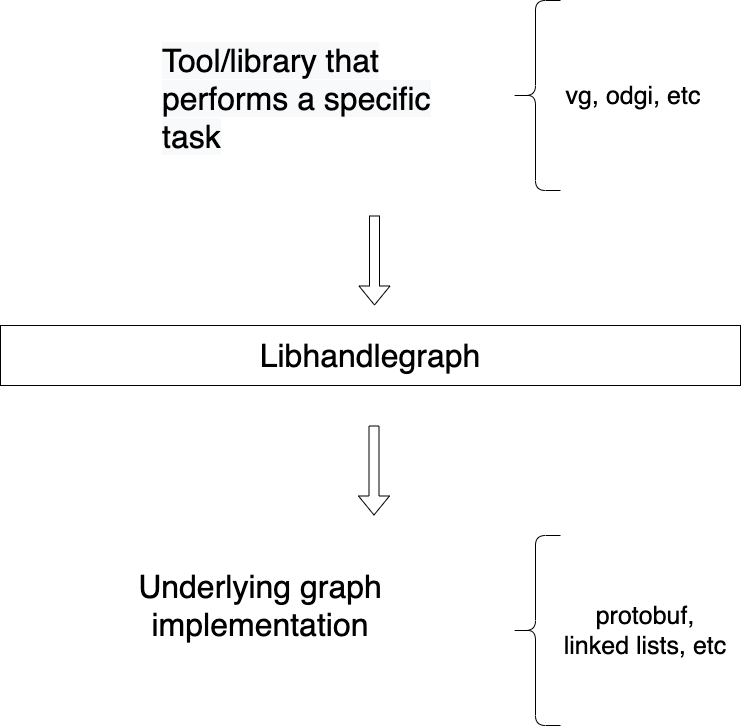
\includegraphics[width=0.7\textwidth]{figures/libhandlegraph.png}
\caption{libhandlegraph...}
\end{figure}

libhandlegraph is primarily used in vg as an abstraction layer over different
backing graph implementations.
It defines a common set of attributes and operations through which we can
manipulate the graph. We can then use the libhandlegraph API as a layer between
an underlying graph implementation and genome graph manipulation tools we plan
on building.

libhandlegraph has python bindings and is now being ported to Rust. In C++ and
Python, it uses the class abstraction while in Rust the trait abstraction.

libbdsg (Optimized bidirected sequence graph implementations for graph genomics)
is a C++ library that provides high performance implementations of sequence
graphs for graph-based pangenomics applications. Tools built on top of this are
PackedGraph (low memory) and HashGraph (high-performance hash tables).
vg is now using libhandlegraph through libbdsg
\cite{eizengaSuccinctDynamicVariation2020}.

\subsubsection{Plaintext graphical representations}
\label{sec:orgd75f170}
In the early 2000s assembly software was dominated by a few end to end assembly
software such as SPAdes, ALLPATHS, ABySS, and SOAPdenovo
\url{https://pmelsted.wordpress.com/2014/07/17/dear-assemblers-we-need-to-talk-together/}.
These end to end tools made it hard to tweak parts of the assembly process which
led to calls (such as \href{https://github.com/pjotrp/bioinformatics}{THE SMALL TOOLS MANIFESTO FOR BIOINFORMATICS}) for small
tools that perform bits of the assembly while using plaintext files as APIs.

An early attempt was FASTG,  an extension to FASTA, which is based on a directed
graph (digraph) and was originally meant to represent variability in the final
output of the assembly process.
It encodes the sequences on arcs/edges and refers to the connection
between sequences as vertices.

Like FASTA, each record contains a header line which follows the pattern
a greater than sign, the edge, the neighbors of the edge and the edge properties.
\(>Edge:Neighbours:Properties;\) where: Edge is the name given to this
edge/sequence, Neighbors is a list of edges or their reverse complements that
follow this edge or the reverse complement of this edge
(indicated by a preceding\textasciitilde{}), and Properties is a list of optional properties
associated with this edge. To facilitate
inversions, the format allows for adjacencies between forward and reverse
complement. Reverse complements are indicated by a prime symbol \('\)
.


\begin{verbatim}
>x:y;
ACGTGAGAT
\end{verbatim}
An example of a FASTG fragment where x represents
a DNA sequence and an edge in the graph. The edge is in turn followed by edge y.
There exists an adjacency from edge x to edge y.

GFA \cite{liMinimapMiniasmFast2016} comes in two versions:
GFA1 (\url{https://gfa-spec.github.io/GFA-spec/GFA1.html}) and
GFA2 (\url{https://gfa-spec.github.io/GFA-spec/GFA2.html}) with GFA2 being a superset
of GFA1.
Unlike FASTG, GFA is a total deviation from the FASTA format aimed specifically
at plaintext representation of genome graphs and able to represent a graph at
all stages of the assembly <citation needed> as well as varying topologies
(can encode bubbles).
Unlike FASTG, it encodes the sequences on the nodes, which it names segments and
has edges as the connections between segments.
Each line must begin with either H (header), S (Segment), F (Fragment), E (Edge),
G (Gap) and G or U (Group) and each token is separated from the next by a tab
(is tab delimited).
It can encode extra detail through fragments which are used to specify a
collection of external sequences or edges which may contain a Dazzler-trace or
a CIGAR string to describe the alignment of the edge.

rGFA \cite{liDesignConstructionReference2020} is GFA extended for reference
(pan)genomes. It is an extension
to GFA with 3 additional tags that indicate the origin of the segment to
provide a unique stable coordinate system as an extension to the linear
reference coordinate. Each segment is associated with one origin which forbids
collapsing of different nodes from one region as would be with a cDBG  in the
graph by design. rGFA disallows overlaps between edges and forbids multiple
edges (more than one edge between the same pair of vertices).
rGFA cannot encode a collapsed graph.
To make use of the reference pangenome graphs
GAF \cite{liDesignConstructionReference2020} is a text format
for sequence to graph alignment.
It’s an extension of PAF \cite{liMinimapMiniasmFast2016}.
It is tab delimited like GFA. \todo{describe the grammar}

\subsubsection{Genome graphs as databases (logic programming)}
\label{sec:org6a05fae}
We can also treat the variation graph as a graph database. For this, SpOdgi
\todo{citation needed} transforms any odgi genome variation graph file into a
SPARQL capable database.

\subsubsection{Visualization}
\label{sec:org296b1d1}
Visualization tools are a core tenet of bioinformatics and science in general.
They help us understand our assemblies and communicate the results with others.
Different tools exist depending on the level of resolution needed and
the size of the graph.

GraphViz \cite{northOnlineHierarchicalGraph2002,ellsonGraphvizDynagraphStatic2004}
is a collection of different graph visualization tools \todo{expound}

Bandage \cite{wickBandageInteractiveVisualization2015}, originally developed for
assembly graph visualization, is a standalone application written for
visualizing assembly graphs.
It allows the visualization of several contigs which they themselves may have
various paths within them.
It uses a force-directed layout via, strength is aesthetic appeal and clearly
communicates components but annotation and navigation aren’t possible.
The major issue is the runtime scalability; force-directed layout has quadratic
or even cubic costs with respect to graph size \todo{cite pantograph docs}.
The Open Graph Drawing Framework library (\url{http://www.ogdf.net/}) is used to
perform the graph layout using the fast multipole multilevel layout algorithm,
which scales well for very large graphs
\cite{hachulLargeGraphLayoutAlgorithms2007}.

It reads a graph in a variety of formats: LastGraph (Velvet), FASTG (SPAdes),
Trinity.fasta, ASQG and GFA and allows the export of a visualization graph
either entirely or a section of it (\url{https://rrwick.github.io/Bandage/}).

MoMI-G \cite{yokoyamaMoMIGModularMultiscale2019}
(MOdular Multi-scale Integrated Genome graph browser)
is a web based genome browser built for the visualization of structural
variants (SVs) in a variation graph and has a chromosome centric view making
it best for prokaryotic, <containing chromosomes> genomes.
It works through a server client web architencture where the client (browser)
makes requests to a backend server that one can set up locally using docker.
It takes as input: a succinct representation of a variation graph in XG format,
read alignment (optional), and annotations (optional).

Sequence tube maps \cite{beyerSequenceTubeMaps2019} is a javascript module that
can be accessed within MoMi-G for the visualization of variation graphs or one
can  build their own custom API to generate the data whose aim is to represent
both structural variation and sequence alignments.
Tube maps were initially built to represent public transportation networks,
London’s iconic Tube Map, \cite{cartwrightamBeckRepresentationLondon2012} which
themselves were inspired by circuit diagrams.

For visualizing large graphs which contain paths, assembly graphs which are de
Bruijn graphs don’t contain paths, it’s recommended to use a pipeline such as …
These break a large graph into “chunks” that can be visualized bit by bit.
Pantograph (2020) is another web based variation graph browser.
It renders the genome graph in a matrix. It reads a variation graph in JSON from
odgi bin.

\todo{Add image of our Household 20 dataset in pantograph}

\newpage
\section{Materials and Methods}
\label{sec:org2f5104c}
\subsection{RSV}
\label{sec:org3e204fe}
We started the experiment with fifty three whole genome sequenced RSV 
positive samples from a twenty five member household code-named household twenty
which was part of a household follow up study in the Kilifi Health and 
Demographic Surveillance System and ran over a six month
period collecting nasopharyngeal swabs twice each week
\cite{munywokiInfluenceAgeSeverity2015,agotiTransmissionPatternsEvolution2017,githinjiAssessingUtilityMinority2018}.

Figure \ref{fig:org9864a9f} from
\cite{githinjiAssessingUtilityMinority2018} shows the temporal infection patterns
of nineteen of the twenty five members of household twenty.

\begin{figure*}[h]
\centering
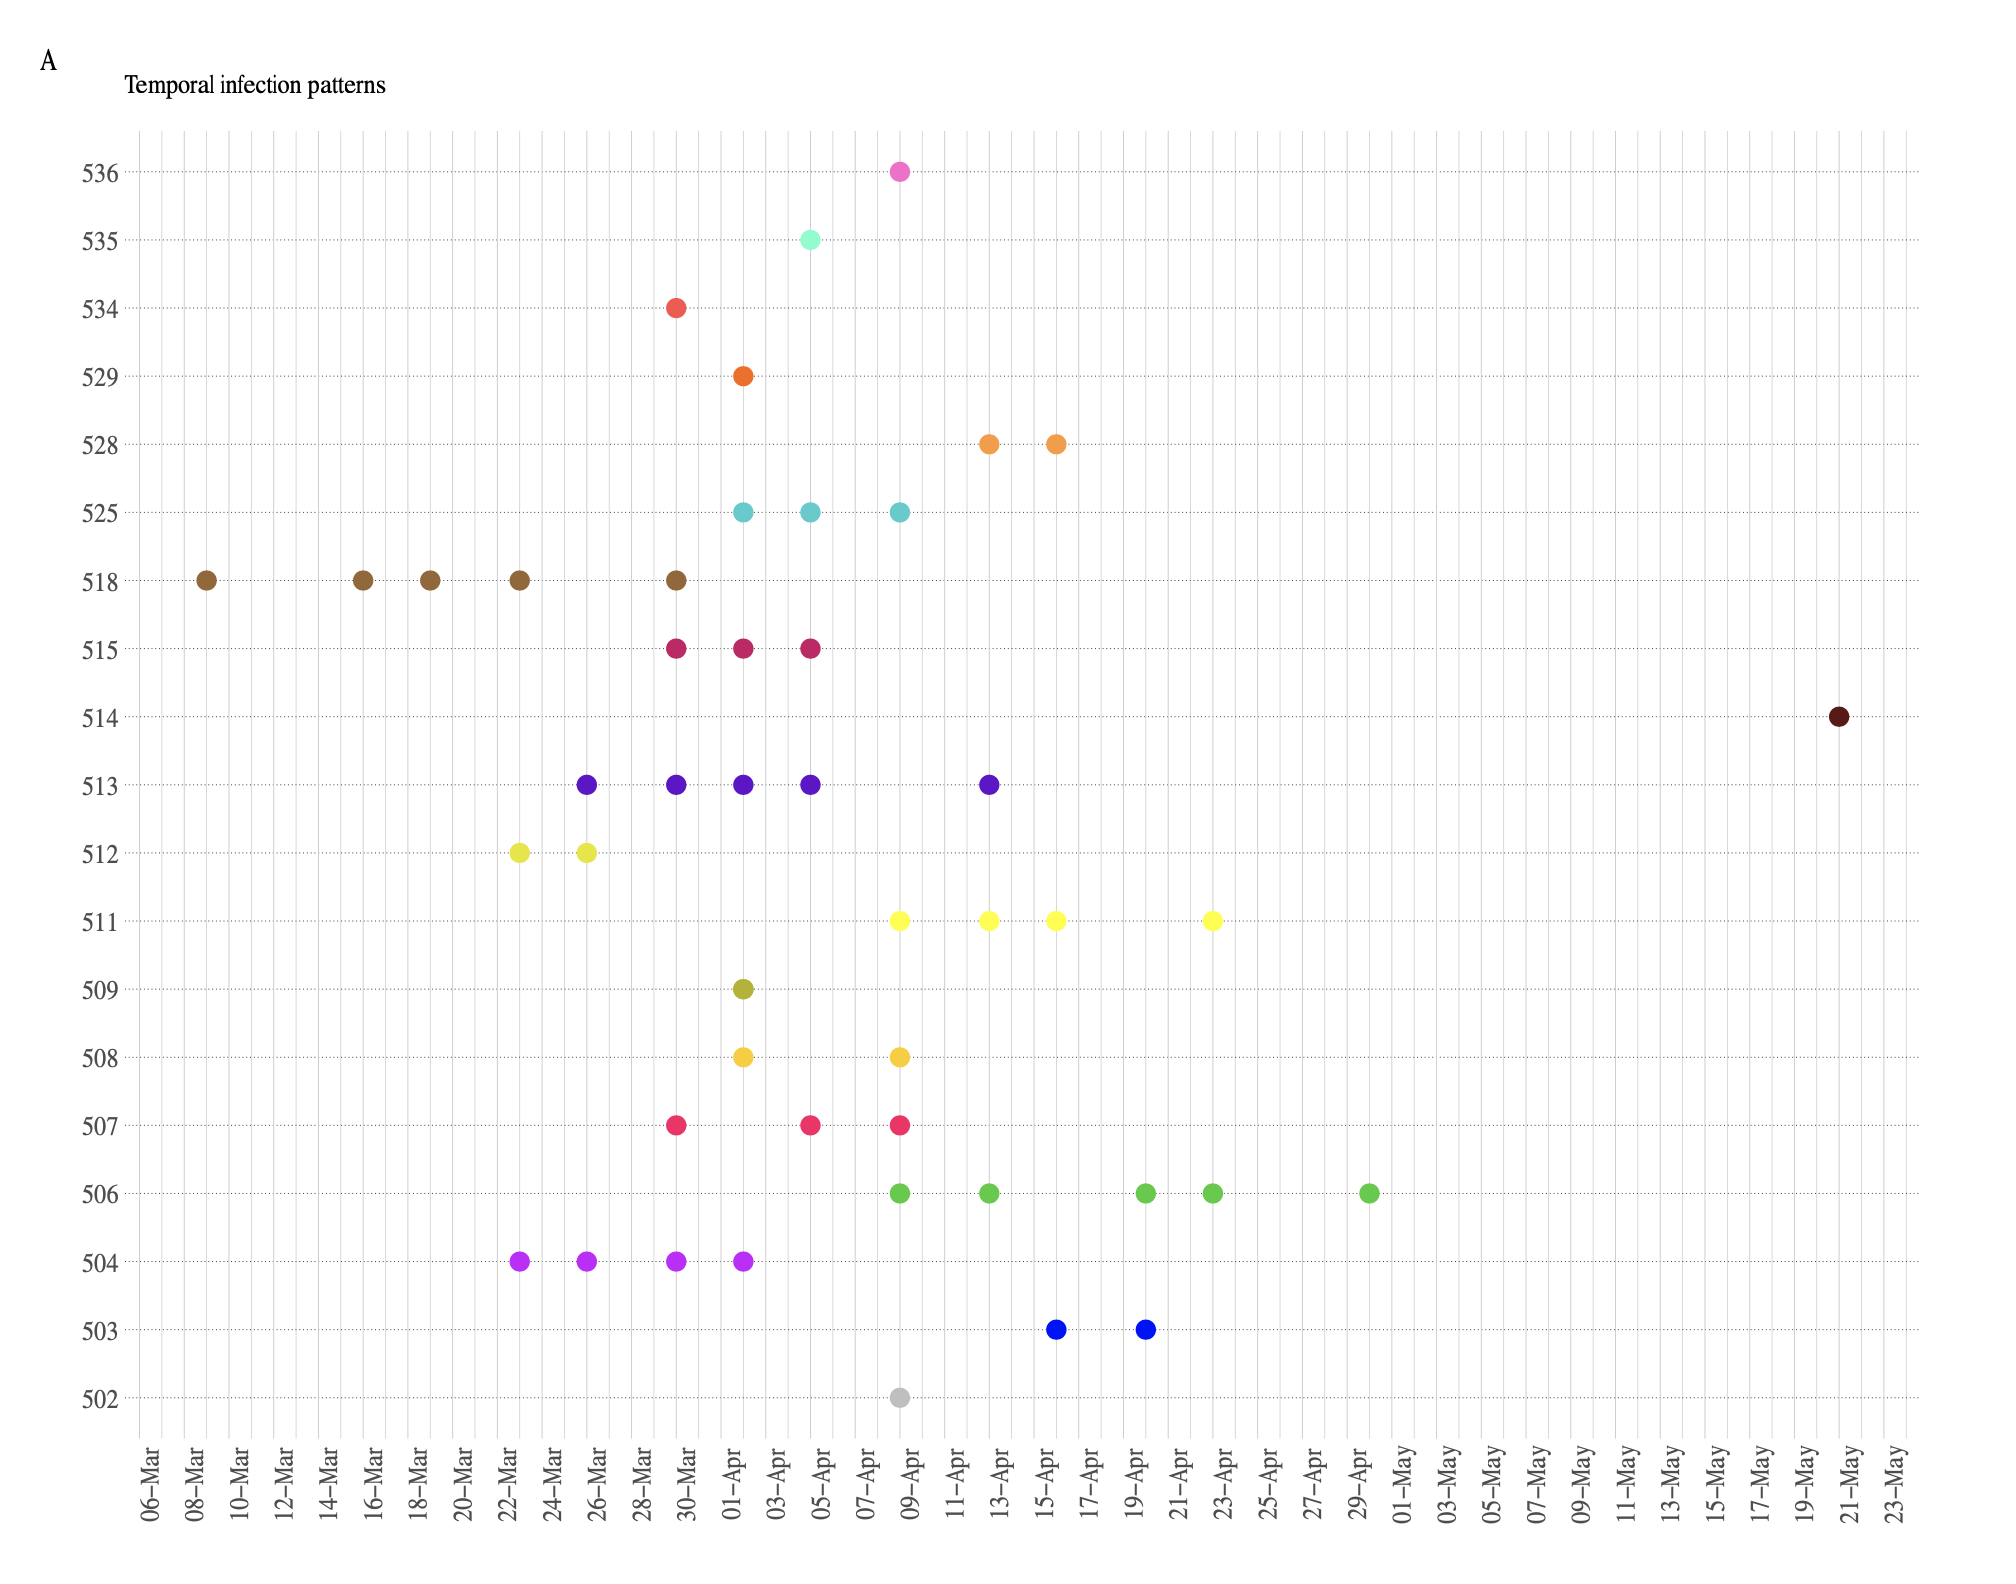
\includegraphics[width=0.75\textwidth]{../Figures/RSV/Githinji_HH_5_temporal_distribution.png}
\caption[Temporal Distribution of RSV Sample Collection]{\label{fig:org9864a9f}
The y-axis shows anonymized individuals represented by integers and unique colors and on the x-axis is the dates on which they were sampled.}
\end{figure*}

\subsubsection{Preprocess and Quality Control}
\label{sec:org70665c4}
We started by removing reads with a phred score below 35 and trimming sequencing
adapters as shown in \ref{sec:orgbcec5a3} then compiled a list 
of the file paths into a text file as shown in \ref{sec:orgc725eae}.

Sequences in two datasets (\texttt{H\_536\_09\_04} and \texttt{H\_506\_13\_04}), specifically those 
stated \ref{sec:org1fd777a}, caused seqwish
(\url{https://github.com/ekg/seqwish}) to crash and were therefore removed from the 
experiment leaving us with 51 samples.

\subsubsection{Construct the Assembly Graph}
\label{sec:org2cfdbda}
We used minia \cite{chikhiSpaceefficientExactBruijn2013} to construct two assembly
graphs with a k-mer length of 31 and varying minimum abundance values.
Given the nature of the dataset (51 samples of approximately 400-500 megabytes 
from a genome that is approximately 15 kilobases in length) it was clear 
that the data was noisy and we had to set a high minimum abundance. 
We varied the minimum abundance values between 1,000 and 2,000 as shown 
in \ref{sec:orge1e0d60} to get a graph of size not greatly exceeding that of
the RSV genome.

A minimum abundance of 1,000 resulted in 157 kilobyte
(approximately 10x the genome size) GFA while a minimum abundance of 2,000 
resulted in a 237 kilobyte GFA (approximately 20x the genome size).
Increasing the minimum abundance from 1,000 to 2,000 reduced the size of the 
resulting graph but on visual inspection seemed to have lost some of 
the variable regions as seen in Figure \ref{fig:org00cc485}.

\begin{figure*}[h]
\centering
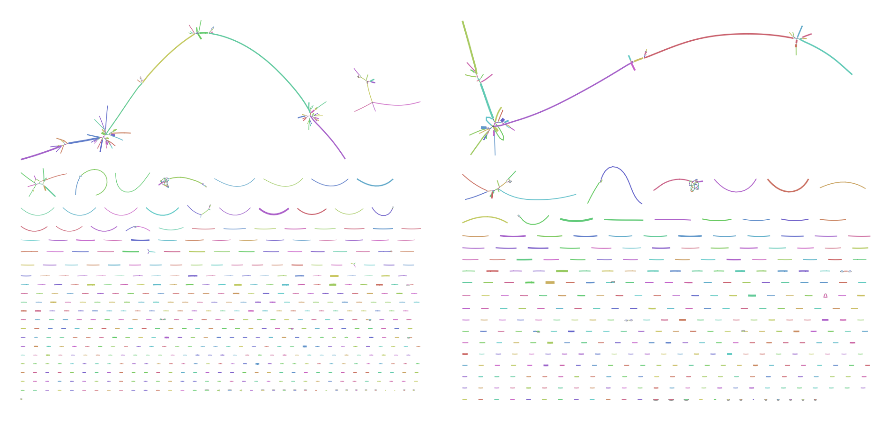
\includegraphics[width=.9\linewidth]{../Figures/RSV/Assembly_Combined.png}
\caption[RSV Assembly Graph]{\label{fig:org00cc485}
An assembly graph of the household 20 samples built using minia and a minimum abundance of 1000 left and 2000 to the right.}
\end{figure*}

\subsubsection{Bluntify the Assembly Graph}
\label{sec:orge10b852}
Going with the 1,000 minimum abundance graph for its increased variability but 
still manageable size we used stark (\url{https://github.com/hnikaein/stark}) to 
bluntify, that is reduce the overlaps on edges,
 \cite{gargGraphbasedApproachDiploid2018} of the graph as shown in
\ref{sec:org8869ee9}.
This yielded a 206 kilobyte GFA that when visualized is seen in Figure
\ref{fig:orgc1d769a}.

\subsubsection{Prepare the graph for mapping with VG}
\label{sec:org4b5af9d}
The bash script in \ref{sec:orgfde9b87} was used to chop and sort the graph
for use with vg \cite{garrisonVariationGraphToolkit2018} which led to the 
variation graph in Figure \ref{fig:orgd339b18}.

\subsubsection{Mapping}
\label{sec:orgc7b402f}
\paragraph{Convert GFA to vg compatible variation graph}
\label{sec:orgfcc71e4}
Using the instructions in \ref{sec:orgea2a9b4}, we induced a vg 
\cite{garrisonVariationGraphToolkit2018} compatible variation graph and output it 
GFA.

\paragraph{Index}
\label{sec:orgda09947}
There was no need to prune the graph because it was small 
(a 62 kilobyte graph.vg) and we wanted to avoid losing complex regions such as 
those with many variants close to each other.
We, therefore, only built an index as in \ref{sec:org43d7006} and got a 61
kilobyte graph (graph.xg) and a 258 kilobyte index (graph.gcsa).

\paragraph{Mapping}
\label{sec:orgb31fccf}
To map each sample against the graph, we used \ref{sec:org3e82afb} to loop through 
each of our interleaved sequences and stored the output GAM files in a 
directory of our specification.

We then verified that the alignments made sense
(a task that is both subjective and a matter of judgment) by converting the GAM 
to GAMP using the instructions in  \ref{sec:org919e7ae} and viewing the JSON.

\subsubsection{Calculate Coverage Across the Graph for Each Sample}
\label{sec:org5a715a5}
We used the script in \ref{sec:org5a35cf6} to generate a coverage vector 196,488 nodes
long in tsv (tab separated values) format.

\subsubsection{Normalization}
\label{sec:orge65c9ca}
The coverage data had a lot of outliers, as shown in Figure
\ref{fig:orgef825ec}, and therefore needed normalization to avoid the outliers
skewing it.

\begin{figure*}[h]
\centering
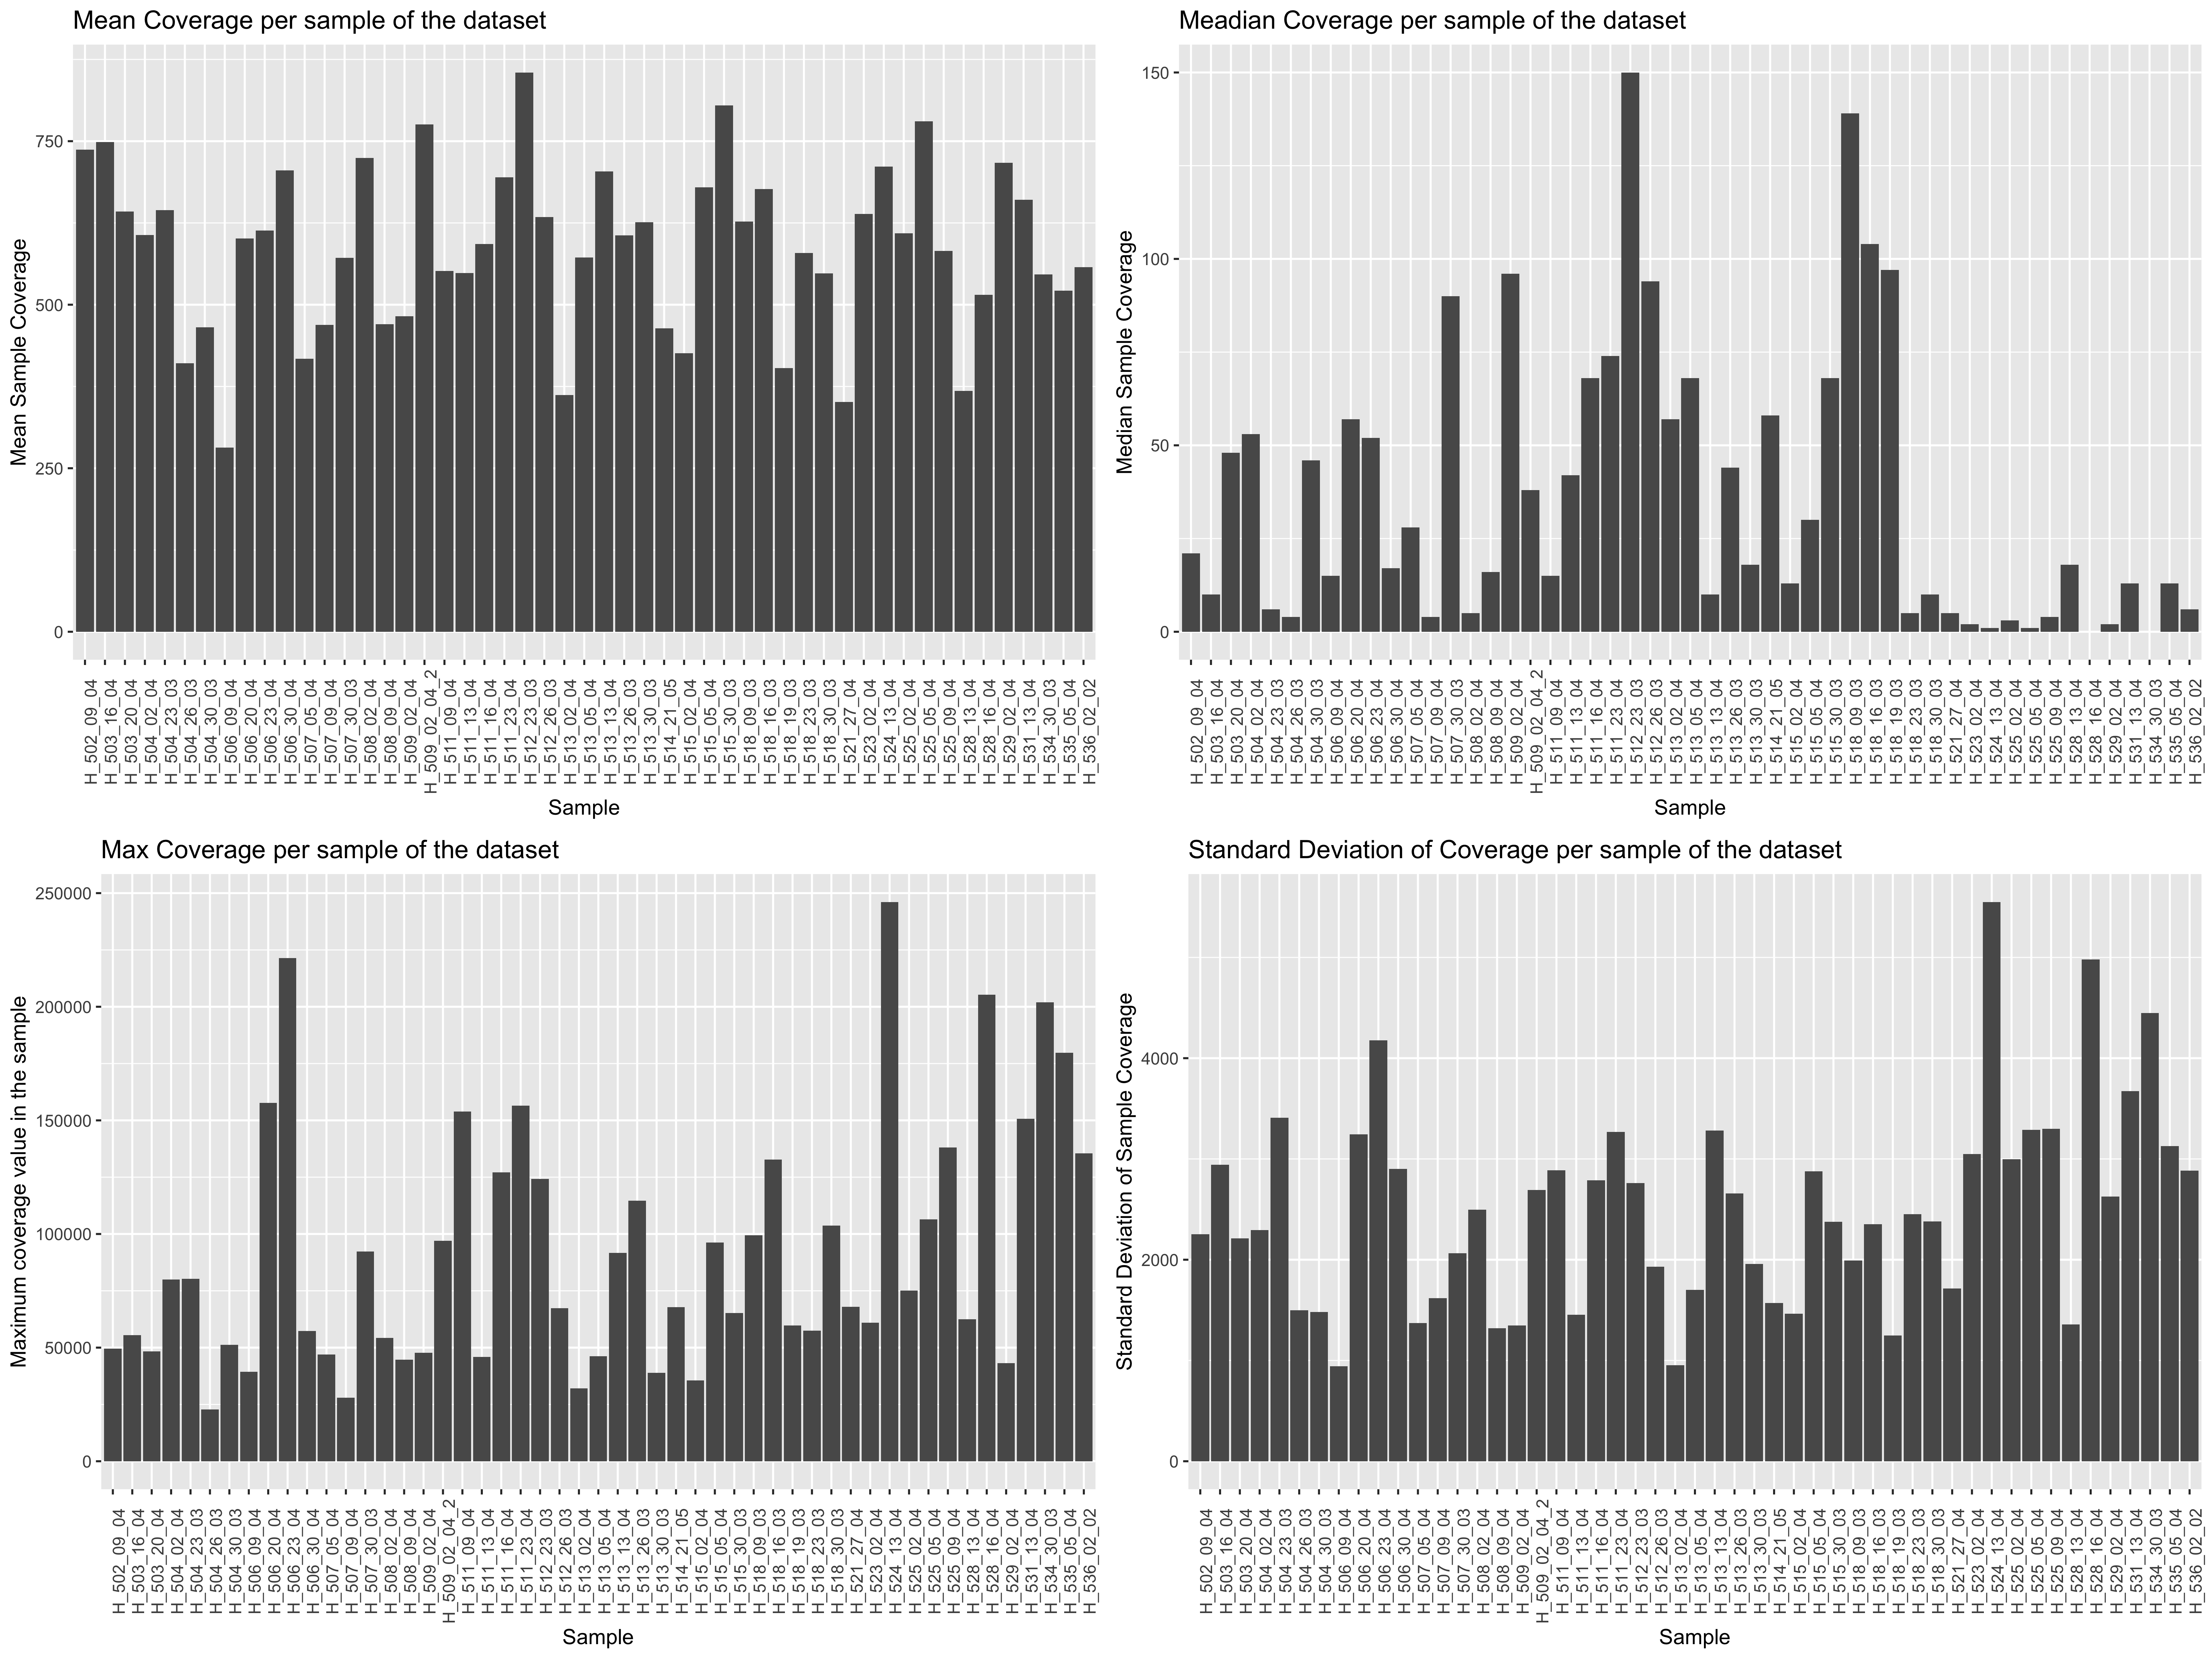
\includegraphics[width=.9\linewidth]{../Figures/RSV/structure_of_coverage_data.png}
\caption[RSV Structure of the Data]{\label{fig:orgef825ec}
Bar graphs of mean, median, maximum and standard deviation of coverage values per sample}
\end{figure*}


We normalized the coverage by setting any coverage value above zero as one and 
left the zero values as zero. This meant that in this analysis, any form of
coverage no matter how deep was valued equally which yielded the heatmap in
Figure \ref{fig:orgd885cc2}.

\begin{figure*}[h!]
\centering
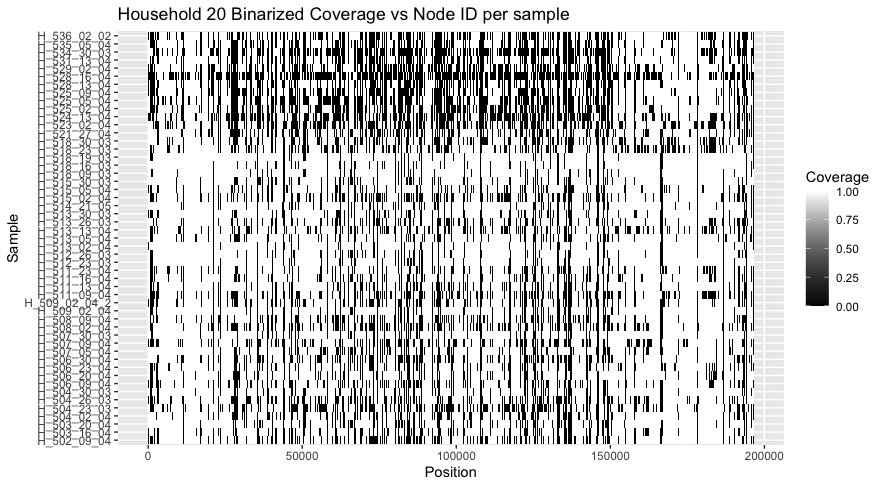
\includegraphics[width=0.7\textwidth]{../Figures/RSV/Heatmap.png}
\caption[RSV heatmap]{\label{fig:orgd885cc2}
A heatmap of the binary normalized coverage vectors of the forty nine RSV samples. On the x axis is the node identifier and the y axis are the individual samples. The light regions indicate coverage while the dark regions indicate no coverage.}
\end{figure*}

\newpage
\subsubsection{Principal Component Analysis}
\label{sec:orgbc9df38}
To make it possible to compare the high dimensional data, we applied Principal 
Component Analysis (PCA) which was able to differentiate each of the samples.
Figure \ref{fig:org41b2633} is a scatter plot of the first and second principal 
components for RSV reads.

\begin{figure*}[h]
\centering
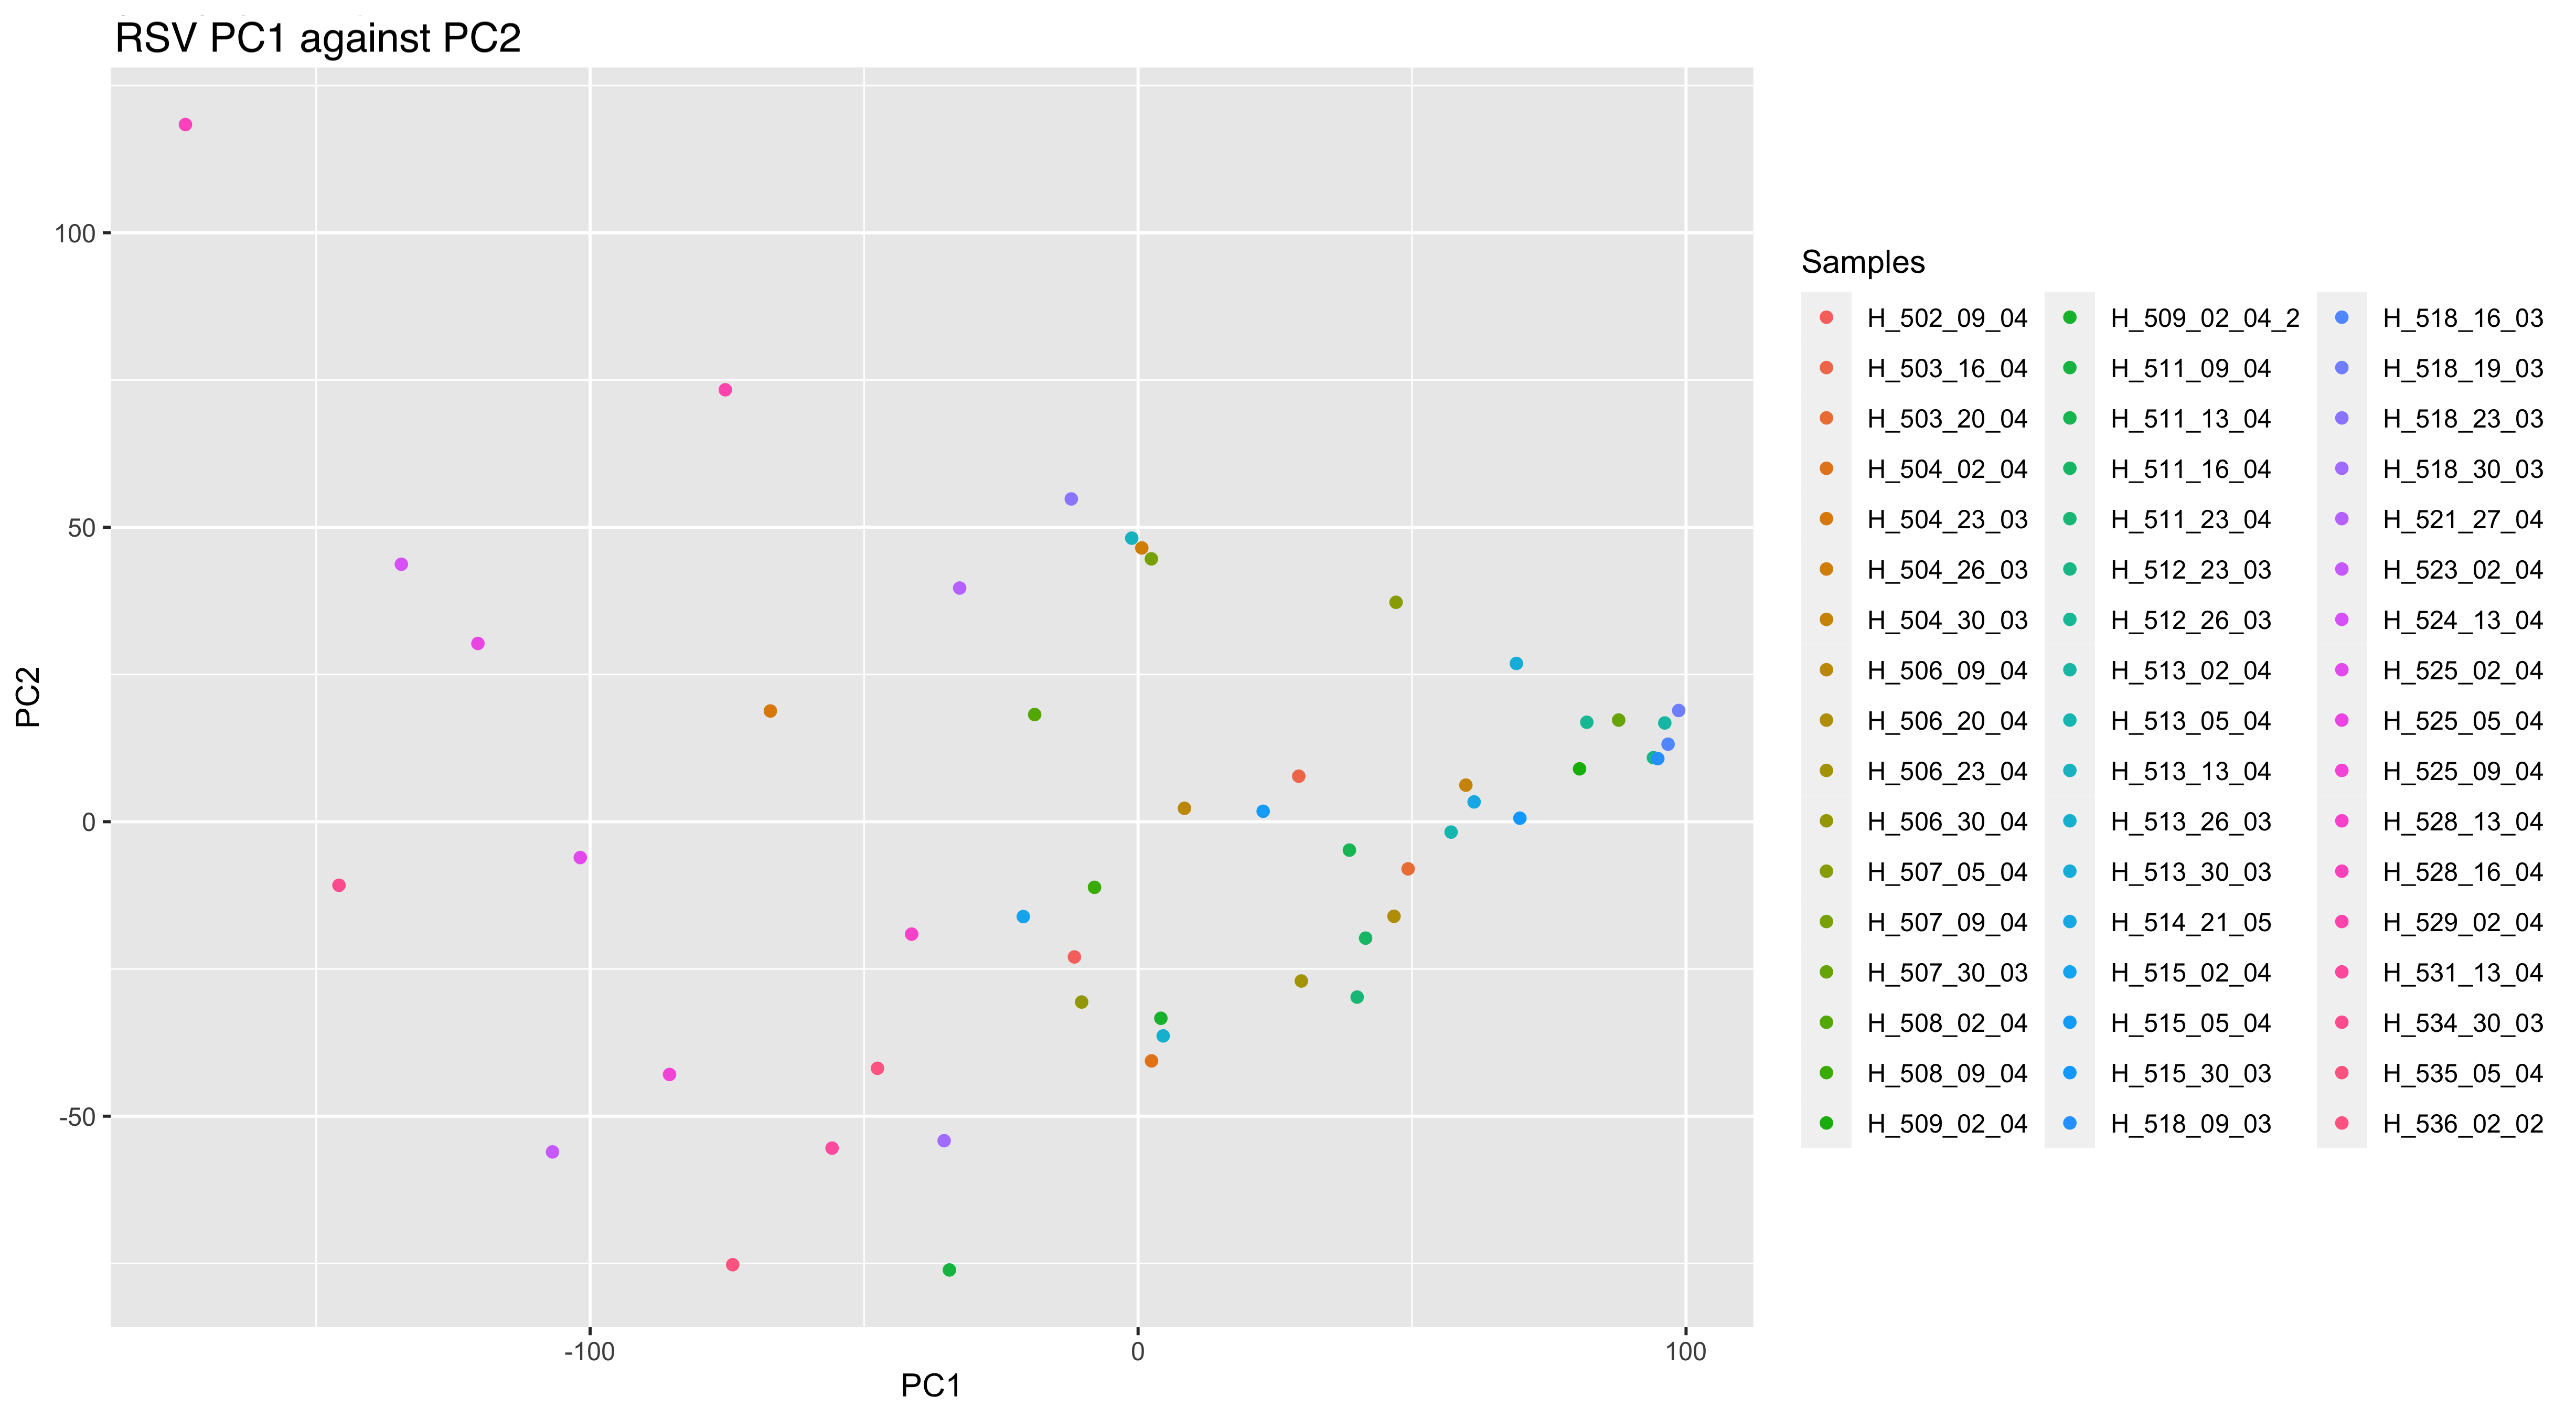
\includegraphics[width=.9\linewidth]{../Figures/RSV/PCA.png}
\caption[RSV PCA]{\label{fig:org41b2633}
A scatter plot of the first and second principal components of the coverage vectors of the forty nine RSV samples.}
\end{figure*}


\begin{figure*}[h]
\centering
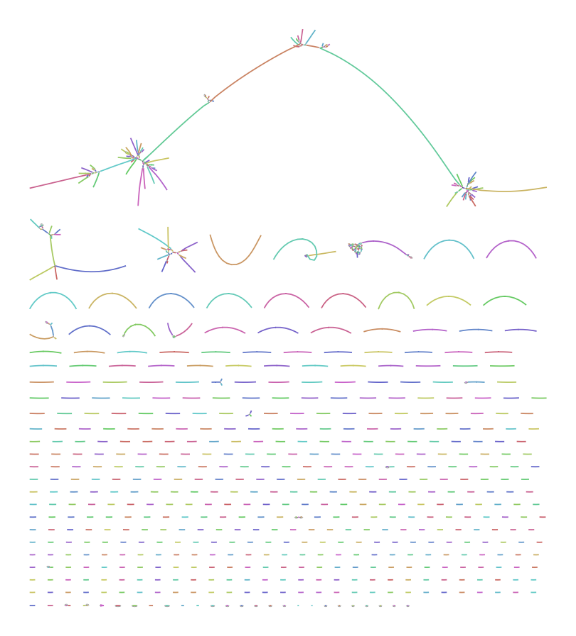
\includegraphics[width=0.75\textwidth]{../Figures/RSV/Assembly_Bluntified.png}
\caption[Bluntified RSV Assembly Graph]{\label{fig:orgc1d769a}
RSV household 20 assembly graph bluntified using stark.}
\end{figure*}

\begin{figure*}[h!]
\centering
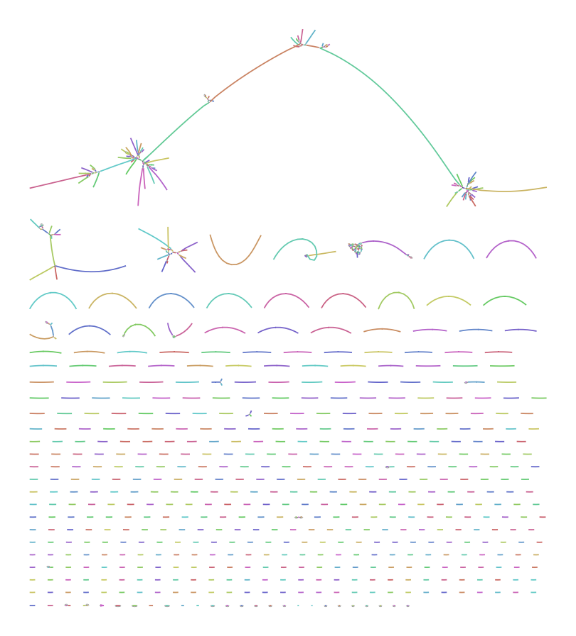
\includegraphics[width=0.75\textwidth]{../Figures/RSV/Assembly_Bluntified.png}
\caption[RSV Variation Graph]{\label{fig:orgd339b18}
The household 20 variation graph after running odgi chop on it.}
\end{figure*}

\clearpage
\subsection{SARS-CoV-2}
\label{sec:orga554126}
Needing to verify that the method in \ref{sec:org3e204fe} properly clusters samples based on 
how close they are genetically we reran the experiment with simulated reads
which have pre-determined and therefore known properties.
The COVID-19 pandemic caused by the Severe Acute Respiratory Syndrome
Coronavirus 2 (SARS-CoV-2) provided a unique opportunity for this. 

\subsubsection{Fetch the Reference}
\label{sec:org30b76c9}
We the fetched latest SARS-CoV-2 \href{https://www.ncbi.nlm.nih.gov/nuccore/1798174254}{reference} as of Jan 17 2020 using the instructions
in \ref{sec:orgc62dd48}.

\subsubsection{Simulate Reads}
\label{sec:org1456132}
Using the reference from our previous step (\ref{sec:org30b76c9}), we simulated 
three sets of 1,000 reads using dwgsim (\url{https://github.com/nh13/dwgsim}).

The first two of the three reads were closely related to the reference and each
other while the third was distantly related from the first two and the
reference.
We achieved this by varying the mutation rate -r (default value 0.0010) while 
keeping the mutation frequency -F (default value 0.5000) constant
\cite{greenSuggestionsConcerningRelationship1995}.

To vary the mutation rates; we used the default mutation rate of 0.0010 for
first two samples which were to be the closely related samples. 
For the third sample which was to be the distant one we increased the mutation 
rate by a factor of 10 to 0.0100. 
The instructions for this are in \ref{sec:orge046742}.

\subsubsection{Construct the Assembly Graph}
\label{sec:orgbada448}
This time we used bifrost \cite{holleyBifrostHighlyParallel2019} to assemble a
colored de Bruijn Graph. 
We did this by saving the file paths to the simulated sequences in a text file
(in our case sequences.txt) then assembled the graph by passing the 
sequences.txt file to bifrost as done in \ref{sec:org98bbb11}.
Figure \ref{fig:org94984fc} shows the assembly graph as visualized in Bandage.

\begin{figure*}[h]
\centering
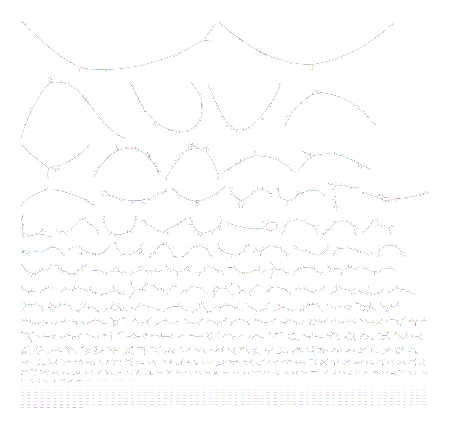
\includegraphics[width=0.75\textwidth]{../Figures/SARS_CoV_2/SARS_Assembly_Graph.png}
\caption[SARS-CoV-2 Assembly Graph]{\label{fig:org94984fc}
A de Bruijn Graph assembled using Bifrost and viewed in Bandage}
\end{figure*}

\subsubsection{Bluntify the Assembly Graph}
\label{sec:org0c3d345}
We then bluntified the assembly graph 
using gimbricate (\url{https://github.com/ekg/gimbricate}) as shown in
\ref{sec:org66af93d}.

\subsubsection{Induce a Variation Graph}
\label{sec:org703a1f4}
We induced a variation graph using seqwish as shown in \ref{sec:org4203a85}.

\subsubsection{Prepare the Graph for Use With VG}
\label{sec:orga3de272}
The GCSA2 \todo{link to literature review} indexer in vg requires nodes to be at
most 1,024 base pairs long.
This meant that we had to reduce the lengths of the sequences in the graph nodes
which was a multistep process.

\paragraph{Build}
\label{sec:orgbc51682}
Build the graph using \texttt{odgi build} as done in \ref{sec:orge429cca}
(pass the \texttt{-s} flag to both build and sort the graph).

\paragraph{Chop}
\label{sec:org5a461ac}
The lengths of the sequences in the nodes were reduced using the instructions in
\ref{sec:org03bcda8}.

\paragraph{Sort}
\label{sec:orgda60103}
Topological order (also known as topological sort) gives us an ascending numbering of nodes which is 
valuable for downstream analysis and serves as a rough coordinate system.
We therefore topologically ordered the graph as in \ref{sec:org53404ea}.

\paragraph{odgi view}
\label{sec:org29fa72a}
We projected the graph into GFA as in \ref{sec:org1ac9d3b} which when visualized in
bandage looks like the one in Figure \ref{fig:org2a9b3d9}.

\begin{figure*}[h]
\centering
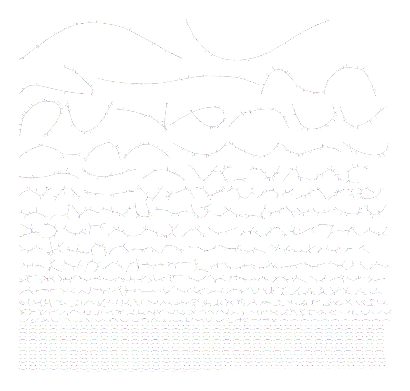
\includegraphics[width=0.75\textwidth]{../Figures/SARS_CoV_2/SARS_Variation_Graph.png}
\caption[SARS-CoV-2 Variation Graph]{\label{fig:org2a9b3d9}
A variation graph that has the length of its nodes chopped using odgi when visualized in badange.}
\end{figure*}

\subsubsection{Mapping}
\label{sec:org6c7b164}
After using odgi to prepare the graph for use with vg
(\ref{sec:orga3de272}), we used vg to map the simulated reads from
each sample to the reference graph which was also a multistep process.

\paragraph{vg view}
\label{sec:org736a5e5}
We used the instructions in \ref{sec:org9e75513} to generate a vg
\cite{garrisonVariationGraphToolkit2018} compatible variation graph. 

\paragraph{vg index}
\label{sec:orge953c0f}
To allow for fast searching of where reads occur in the graph, we indexed the 
graph using the code in \ref{sec:org895f7dc}.

\paragraph{vg map}
\label{sec:org8b62418}
We mapped the reads from each sample (1, 2 and 3 from \ref{sec:org1456132}) to the 
graph which were output as alignments to the graph in the form of GAM files. 

\subsubsection{Calculate Coverage Across the Graph for Each Sample}
\label{sec:org31f1f58}
We then used vg pack to get a coverage vector for each sample as done in 
\ref{sec:orgfeb089b}.

A coverage vector is a table of detailing how deeply reads are align to a 
graph and therefore is quantified as the amount of coverage per node in the graph.

Figure \ref{fig:org115ee46} shows a condensed view of the 106,331 feature
wide coverage vector for the three samples visualized as a pandas dataframe.

\begin{figure*}[h]
\centering
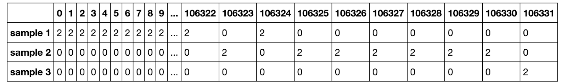
\includegraphics[width=0.75\textwidth]{../Figures/SARS_CoV_2/SARS_Coverage_Vector.png}
\caption[SARS-CoV-2 Coverage Vector]{\label{fig:org115ee46}
The coverage vector from vg visualized as a pandas dataframe.}
\end{figure*}

\subsubsection{Normalization}
\label{sec:orgda9ee55}
The SARS-CoV-2 data had low variance between coverage values with a maximum of 
coverage value 16 (and a minimum of 0) as we can see in the heatmap in Figure
\ref{fig:org96de0f4} and therefore didn’t need normalization.

\begin{figure*}[h!]
\centering
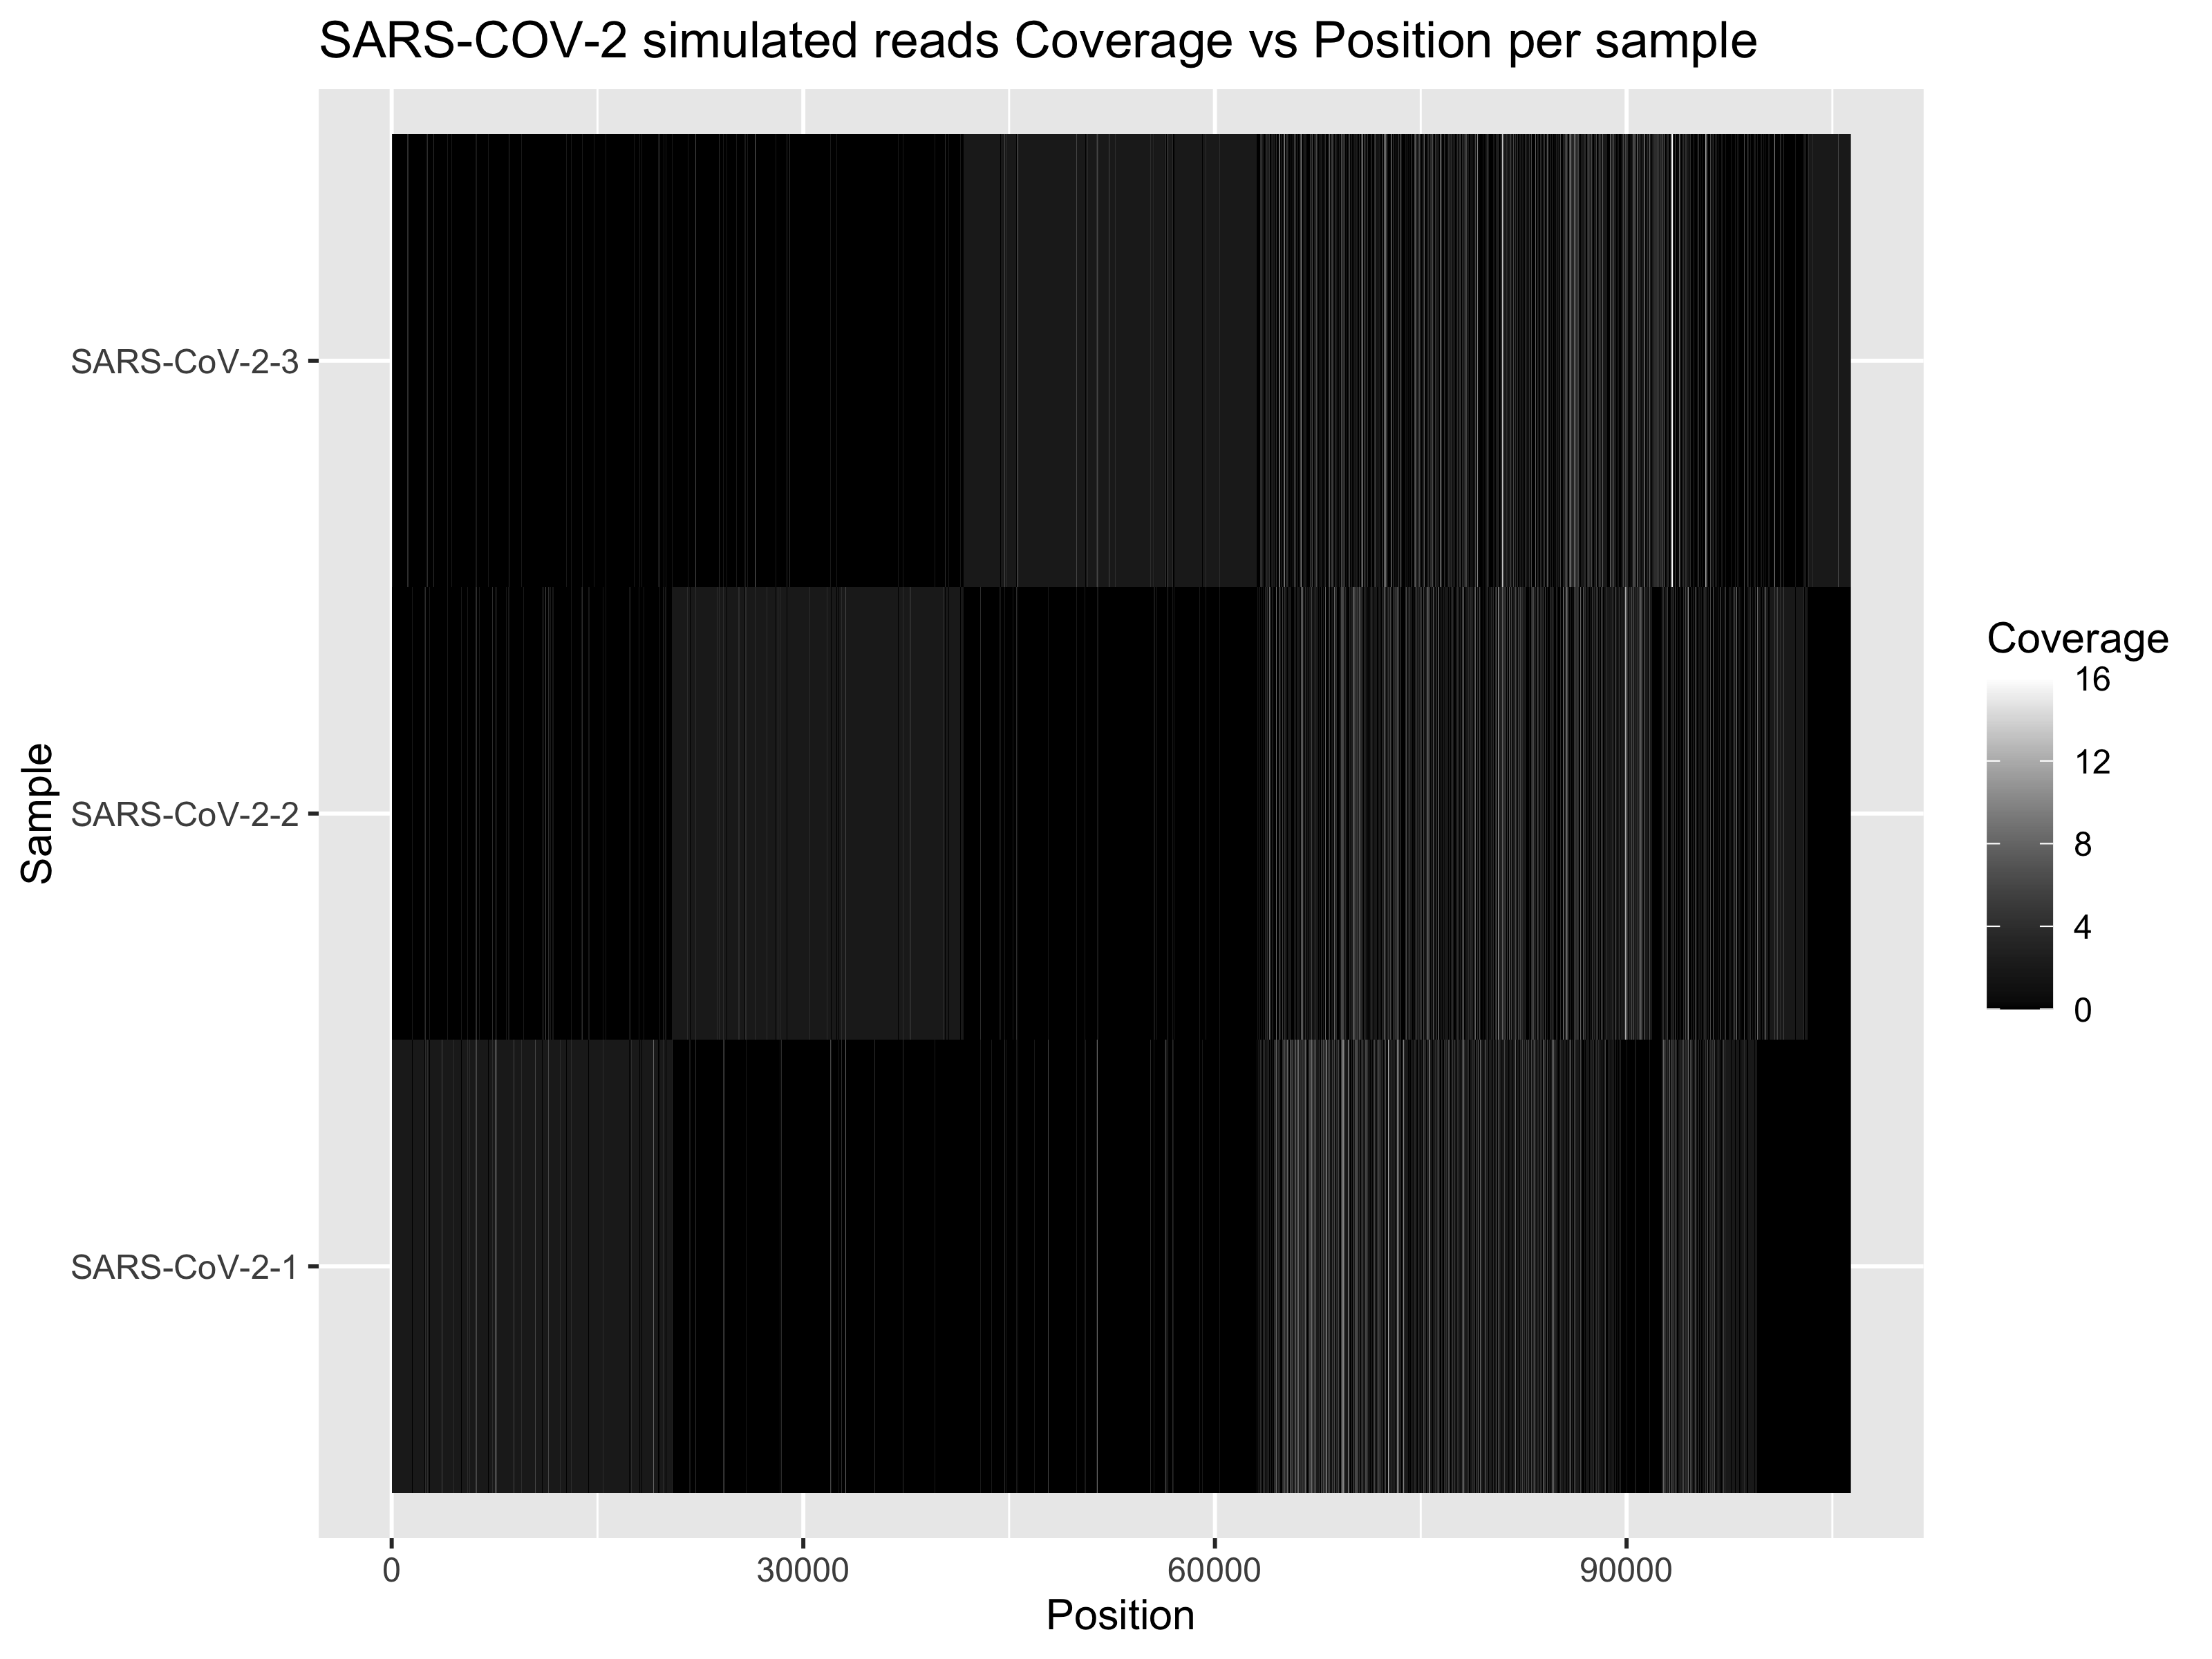
\includegraphics[width=0.75\textwidth]{../Figures/SARS_CoV_2/Heatmap.png}
\caption[SARS-CoV-2 heatmap]{\label{fig:org96de0f4}
A heatmap showing the coverage of each of the samples in one plot. of the coverage of each of the SARS-COV 2 samples. The node identifier of the ordered graph is on the x axis while the number of nodes it mapped to that node identifier is on the y axis.}
\end{figure*}

\newpage
\subsubsection{Principal Component Analysis}
\label{sec:org87548f3}
To make it easier to compare the high dimensional data, we applied principal 
component analysis which was able to differentiate each of the samples as shown
in Figure \ref{fig:org42a605e} as a scatter plot of our PCA, specifically the first and 
second principal components.

\begin{figure*}[h]
\centering
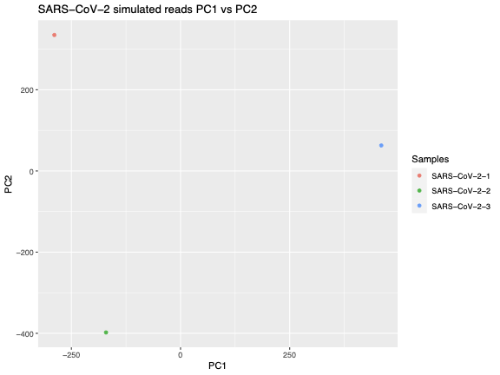
\includegraphics[width=0.75\textwidth]{../Figures/SARS_CoV_2/PCA.png}
\caption[SARS-CoV-2 PCA]{\label{fig:org42a605e}
A scatter plot of the first and second principal components of the coverage vectors of the 3 SARS COV 2 samples.}
\end{figure*}

\clearpage
\section{Results}
\label{sec:orgab52320}
We generated phylogenetic trees based on the distance matrices of i) the first 
principle component ii) the first five principal components which had different 
branch lengths but overall similar topology depending on whether we used the 
first or the first five principal components. 

It is worth noting that both rooted and unrooted trees can be generated by this
method despite us only showing rooted trees. Moreover, other principal
components could have been used but we preferred to use the ones that gave a 
more parsimonious tree.

\todo{Any effects from using different tools for assembly and bluntification?}

\subsection{RSV}
\label{sec:org4ceece2}
When using the first five principal components we generated a tree shown in 
\ref{fig:org5c0bf19} that was more parsimonious.

When using the first principal component we got a tree that seemed to visually
depict a linear relation between the samples in two clades shown in
\ref{fig:orga9c618e}.

Even though the trees from the first or the first five principal components 
have a similar overall topology they have different branch lengths. 
We attribute the maximized branch length in \ref{fig:orgf894e9d} and 
\ref{fig:orga9c618e} to the
first principal component being the one that differentiates the data the most.
It seems that \ref{fig:org175290f} and \ref{fig:org5c0bf19} gave a more realistic
estimation of evolutionary distance.

\subsection{SARS-CoV-2}
\label{sec:org6974dc8}
The differentiation was in accordance with the mutation rates we set when 
\todo{are the mutation rates in the tree exactly in accordance with what we set?}
generating the reads where samples 1 and 2 were closer to the reference and each
other than the sample that allowed for the generation of the dendrogram as shown 
in \ref{fig:orgf894e9d} and \ref{fig:org175290f}.

\begin{landscape}
\begin{figure*}
\centering
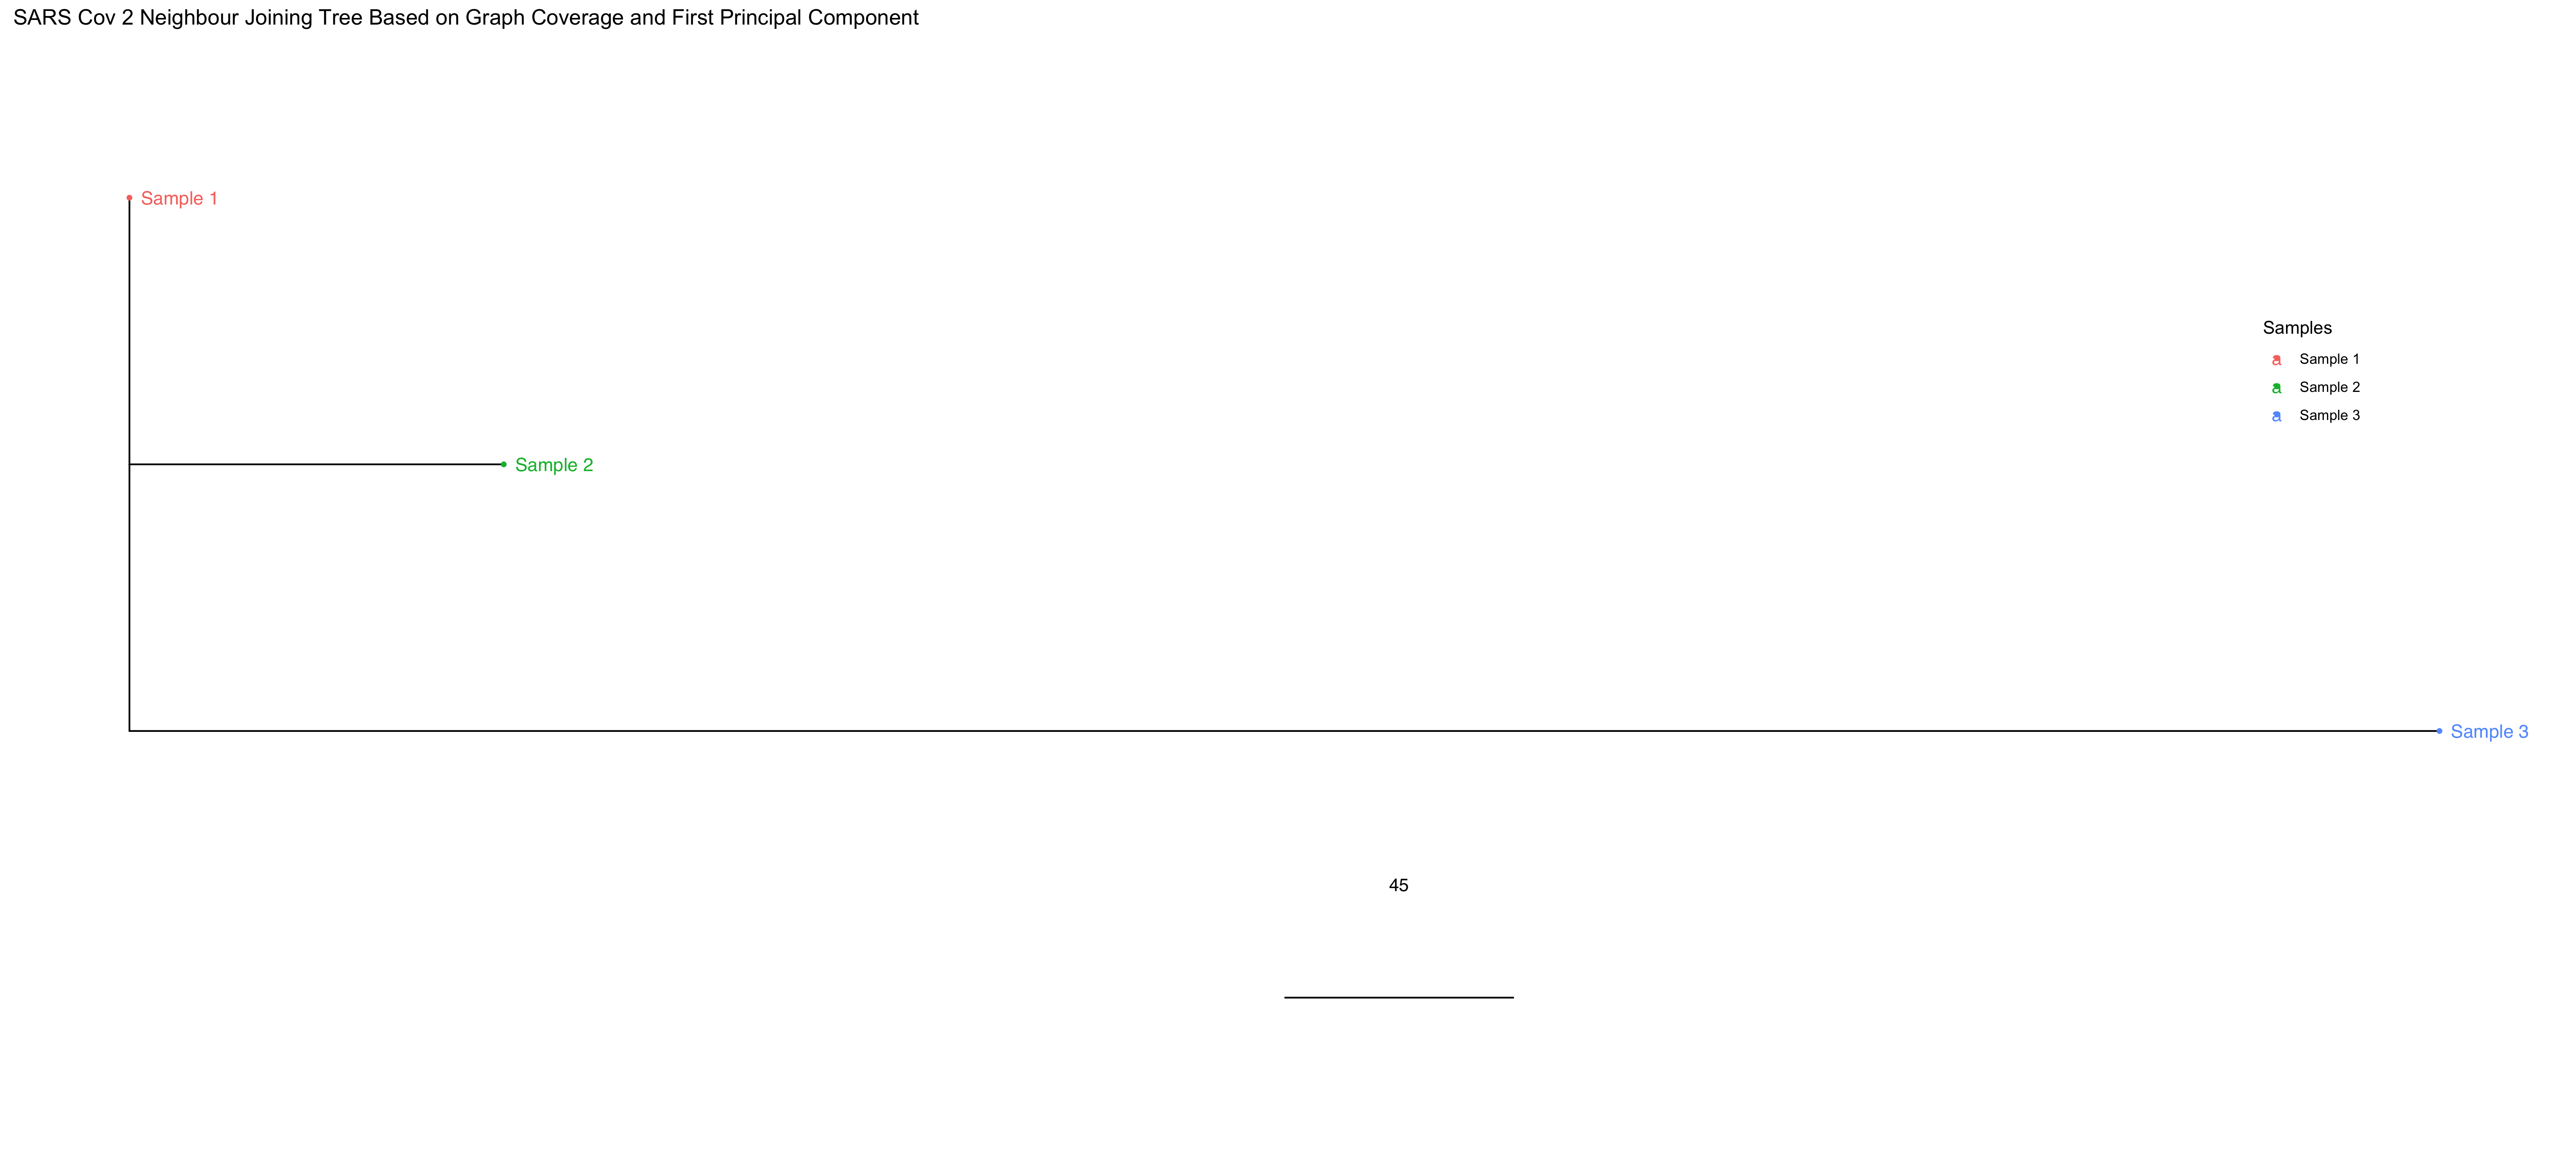
\includegraphics[width=.9\linewidth]{../Figures/SARS_CoV_2/SARS_CoV_2_first_principal_component_nj_tree.png}
\caption[SARS-CoV-2 PC1 cladogram]{\label{fig:orgf894e9d}
A cladogram generated through neighbour joining  of a distance matrix of the first five  principal components of the coverage vector.}
\end{figure*}
\end{landscape}

\begin{landscape}
\begin{figure*}
\centering
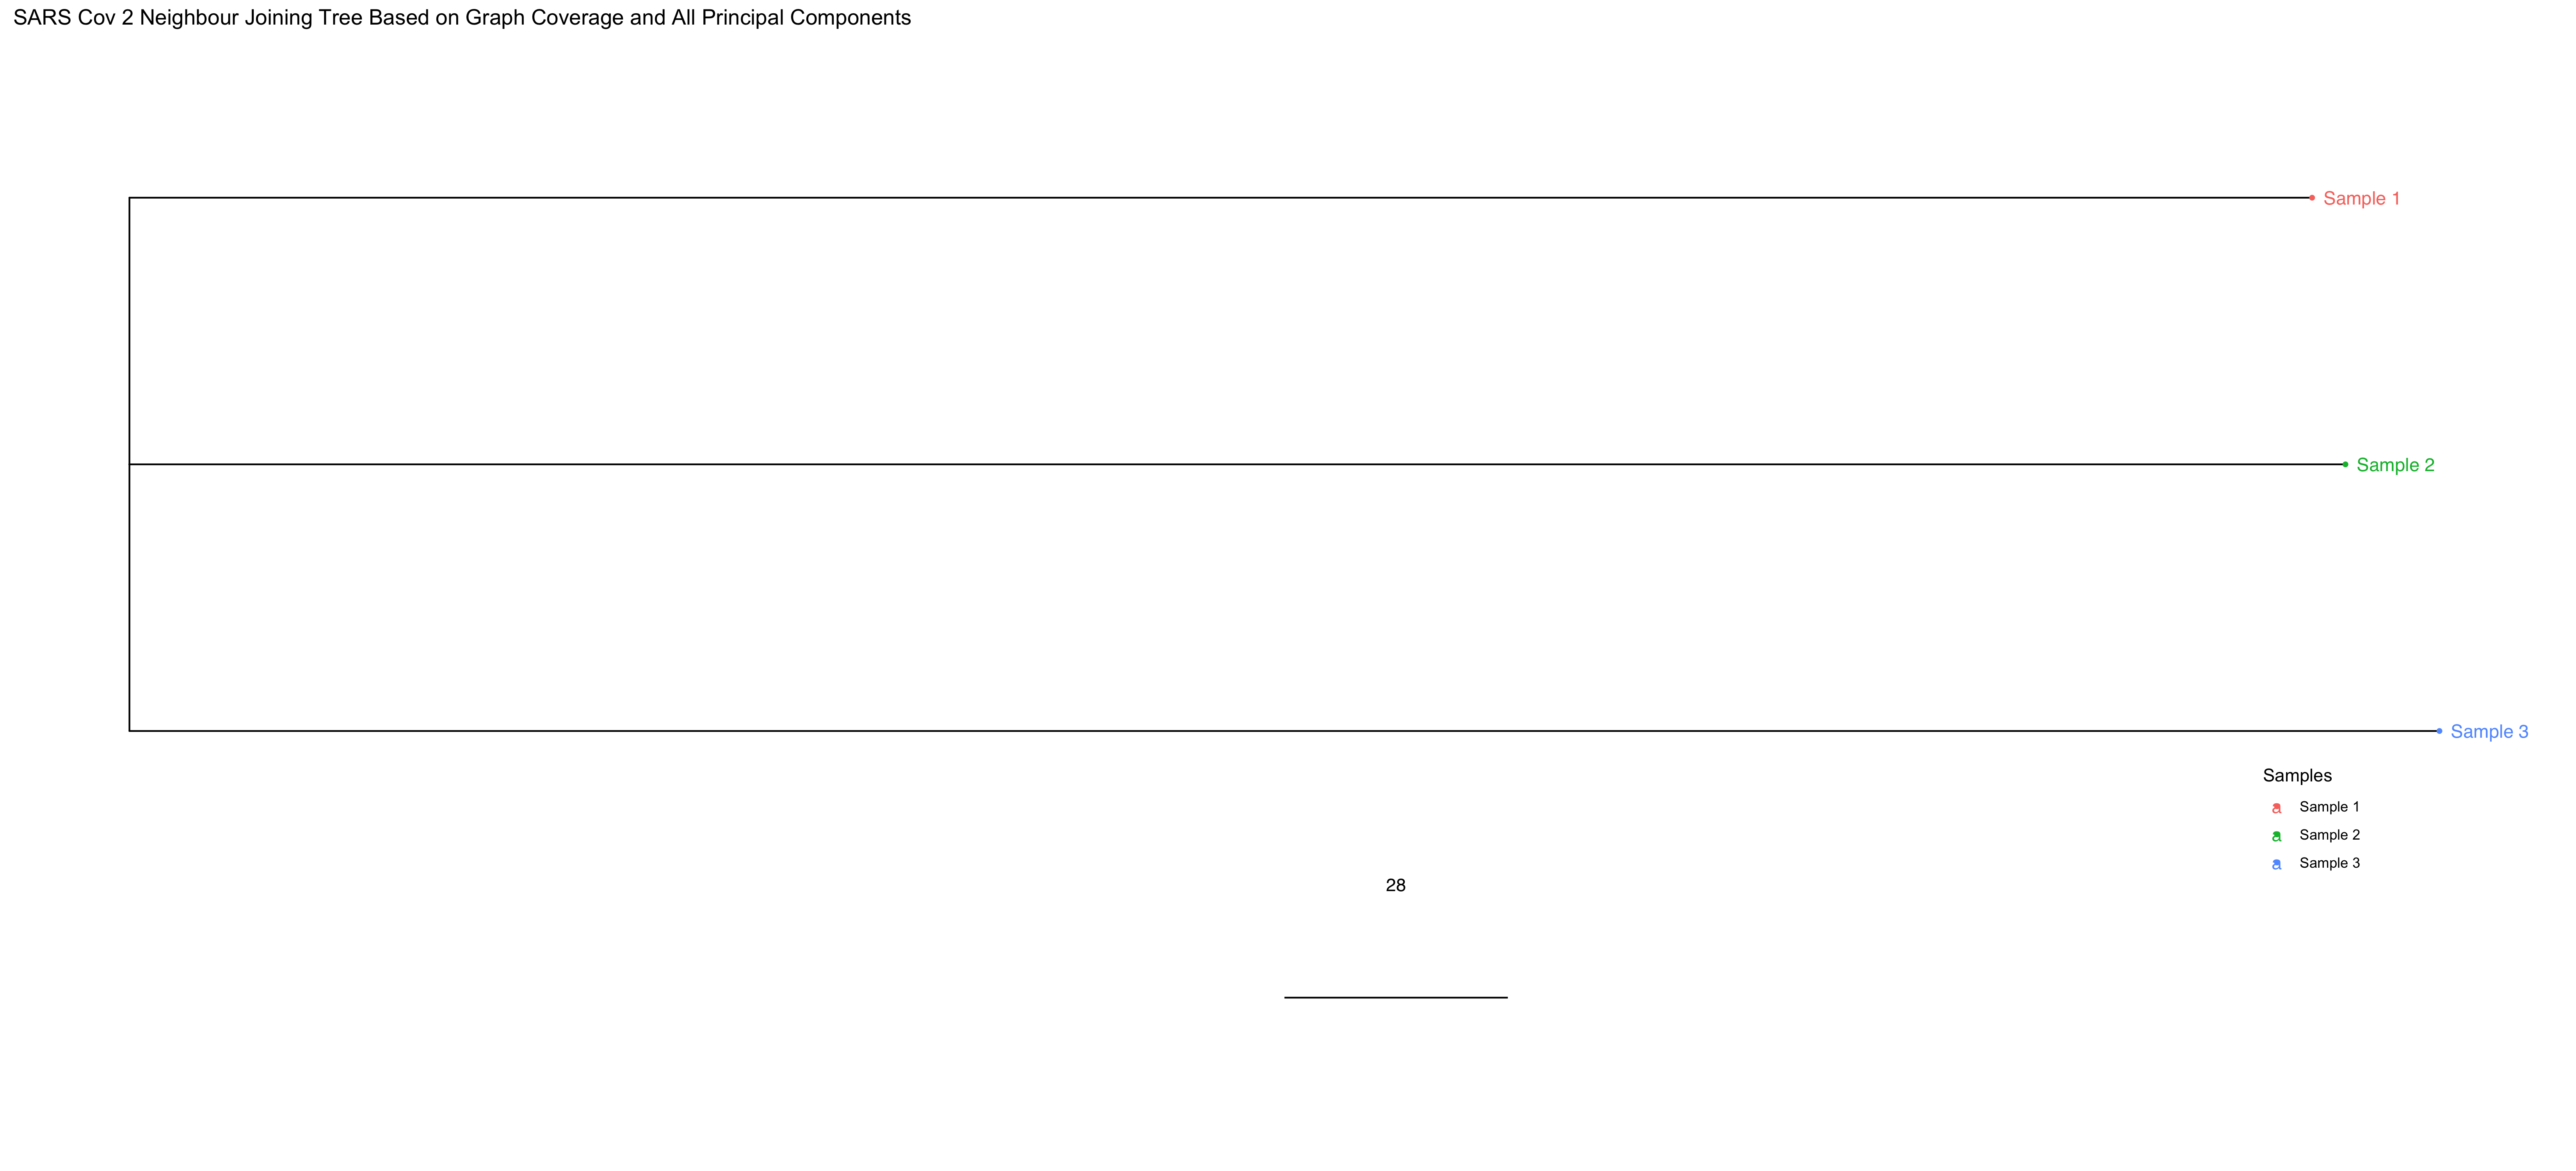
\includegraphics[width=.9\linewidth]{../Figures/SARS_CoV_2/SARS_CoV_2_all_principal_components_nj_tree.png}
\caption[SARS-CoV-2 PC1 to PC5 cladogram]{\label{fig:org175290f}
A cladogram generated through neighbour joining  of a distance matrix of the first principal component of the coverage vector.}
\end{figure*}
\end{landscape}


\begin{landscape}
\begin{figure*}
\centering
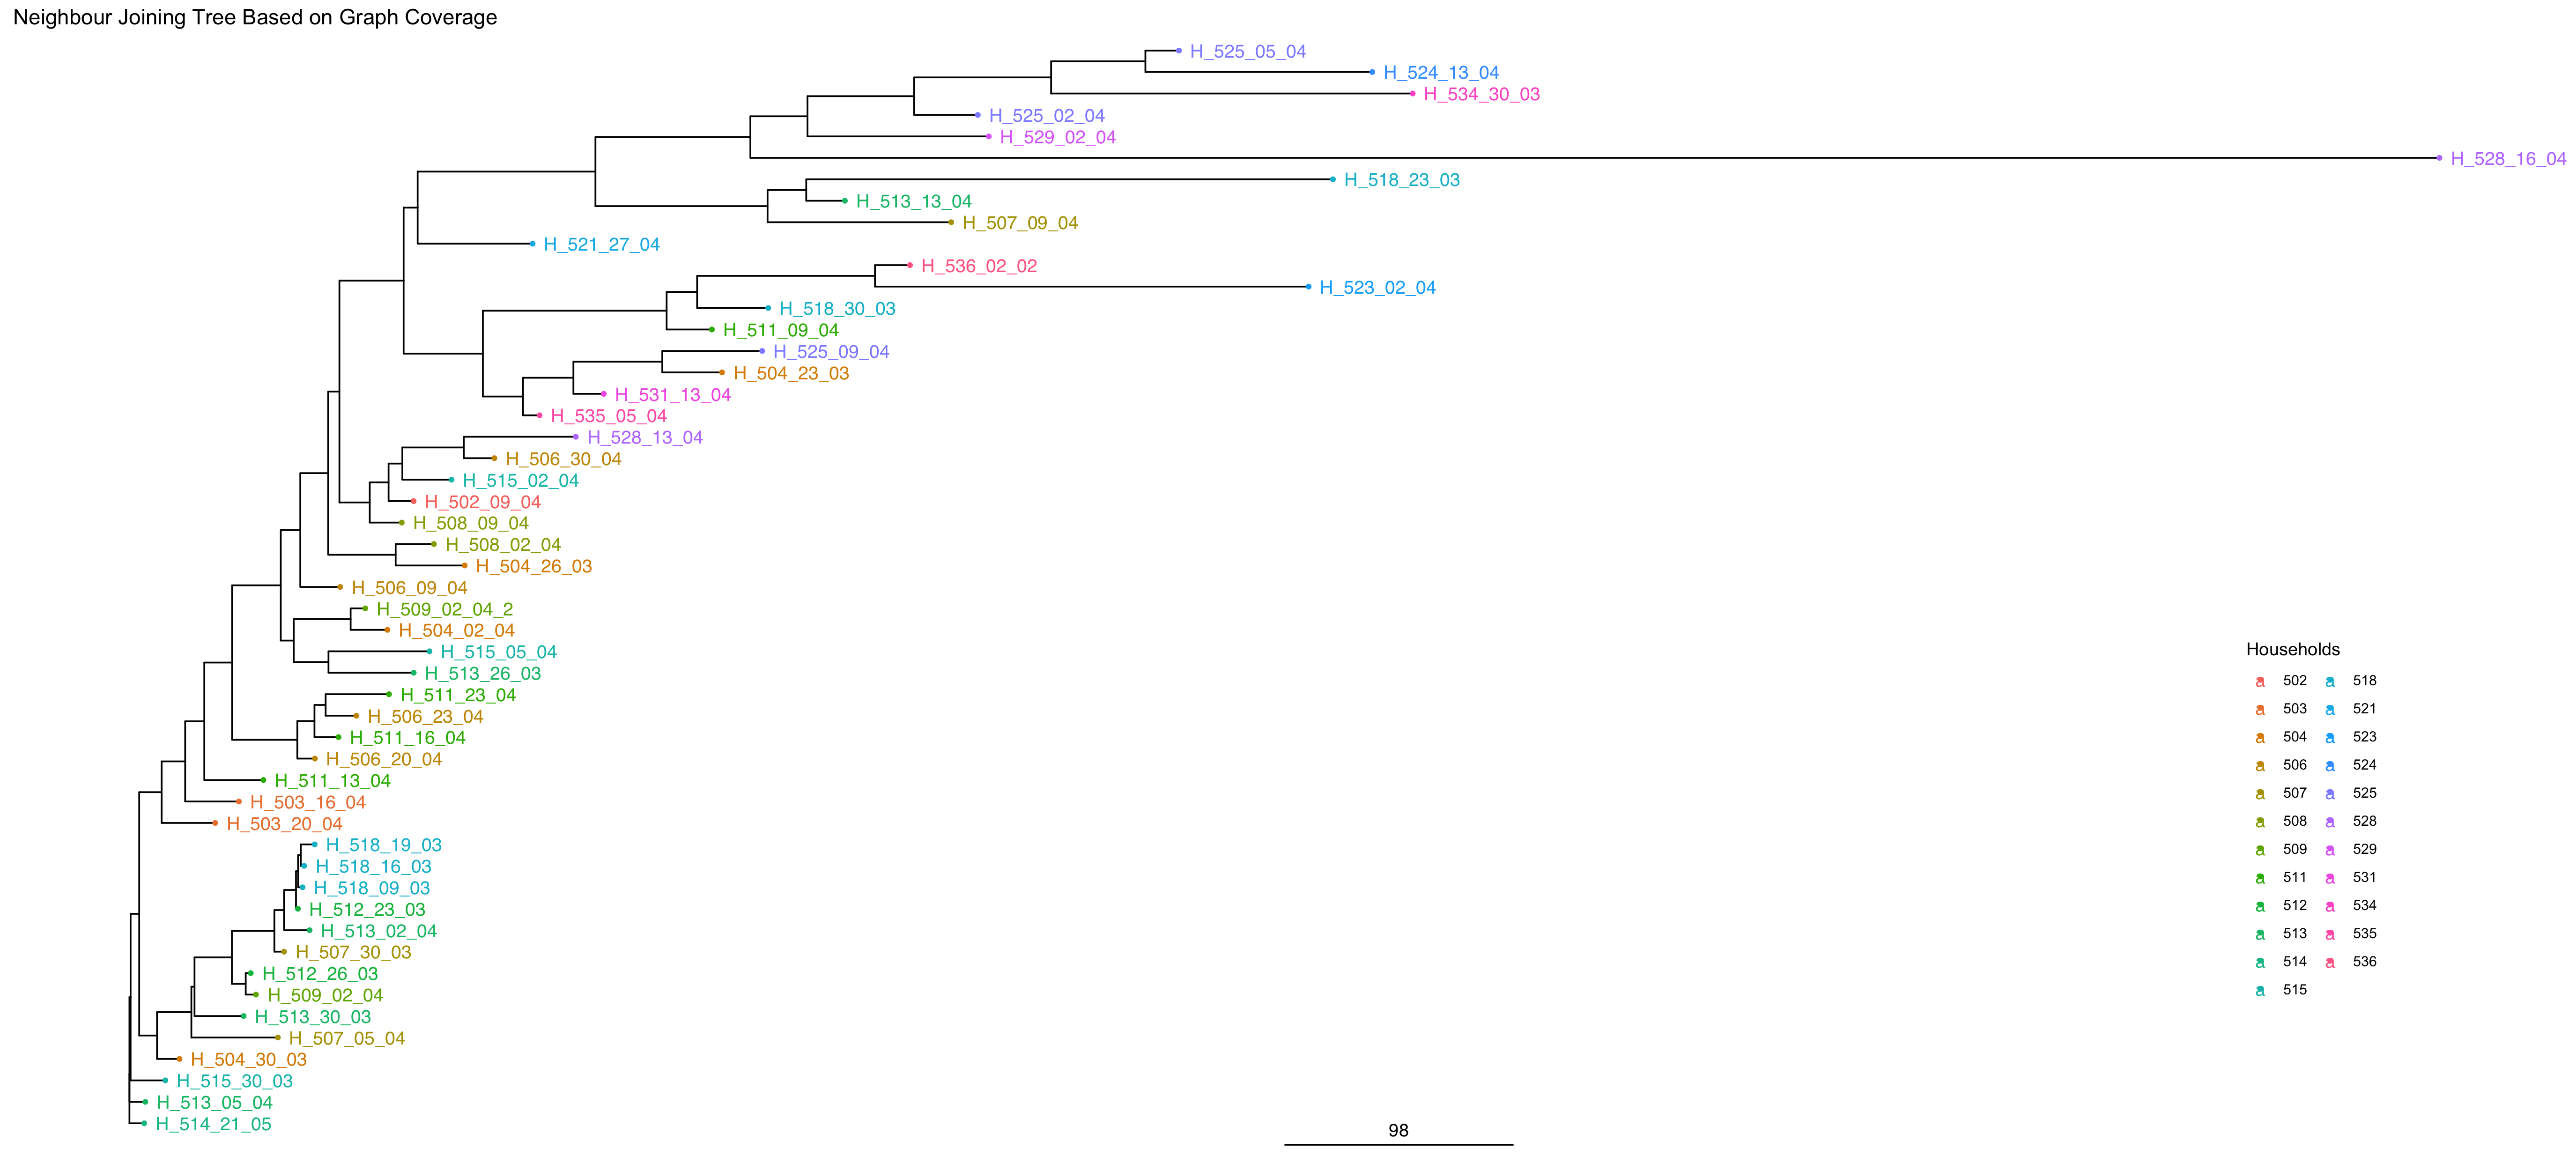
\includegraphics[width=.9\linewidth]{../Figures/RSV/HH20_all_principal_components_nj_tree.png}
\caption[RSV PC1 cladogram]{\label{fig:org5c0bf19}
A rooted cladogram of RSV generated through neighbour joining of a distance matrix of the first five principal components from a principal component analysis of each of the sample’s coverage vectors.}
\end{figure*}
\end{landscape}

\begin{landscape}
\begin{figure*}
\centering
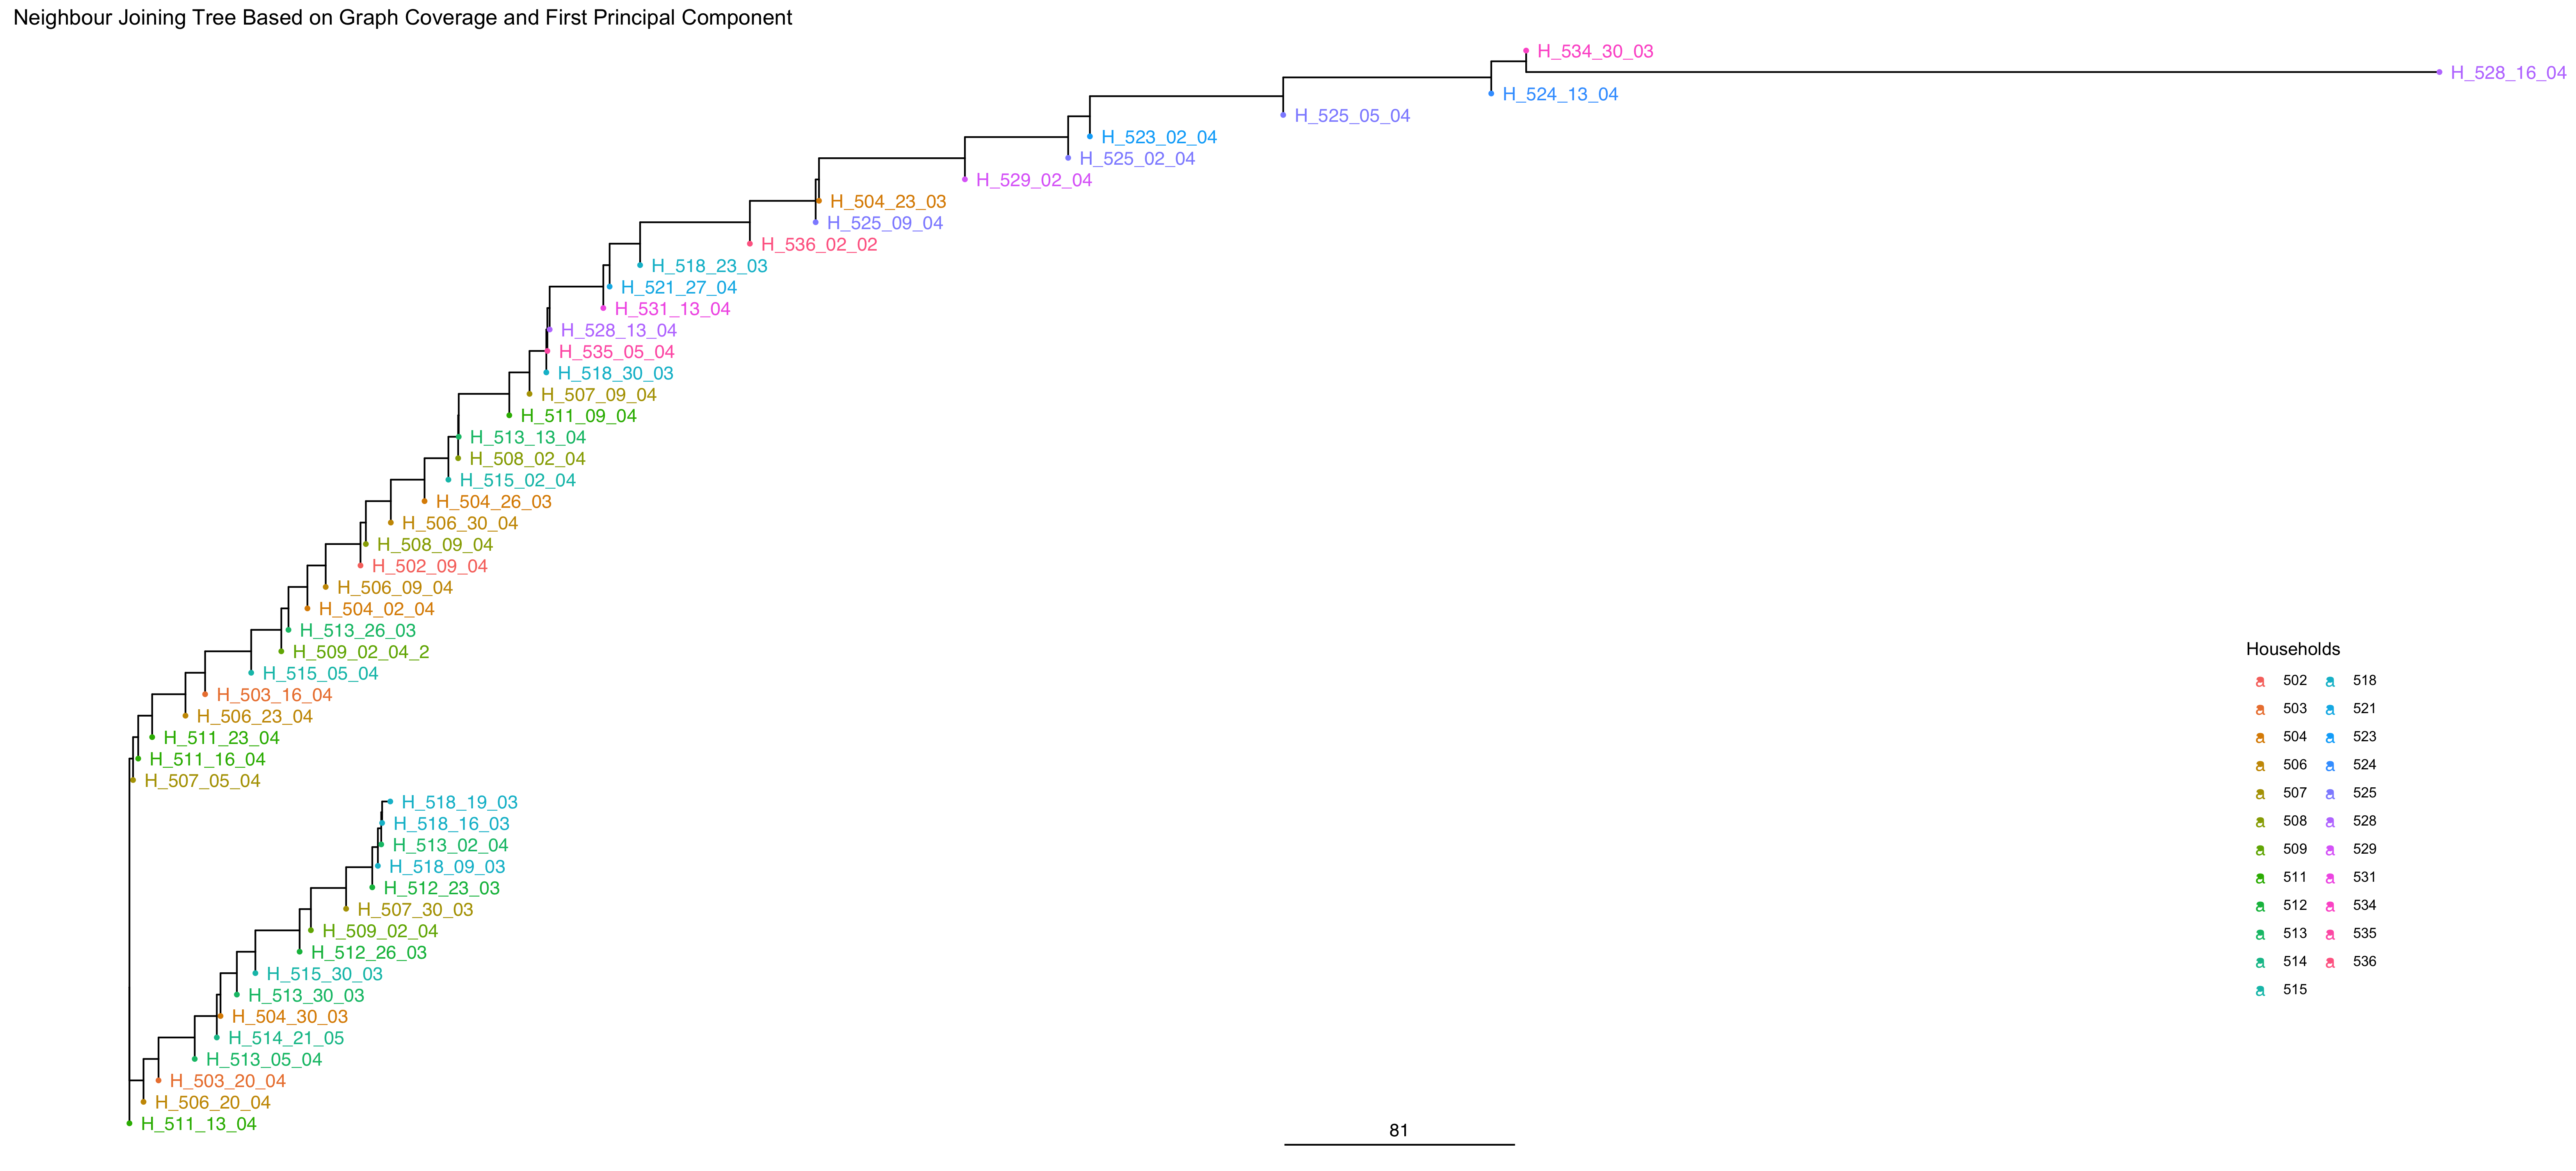
\includegraphics[width=.9\linewidth]{../Figures/RSV/HH20_first_principal_component_nj_tree.png}
\caption[RSV PC1 to PC5 cladogram]{\label{fig:orga9c618e}
A rooted cladogram of RSV generated through neighbour joining of a distance matrix of the first principal component from a principal component analysis of each of the sample’s coverage vectors.}
\end{figure*}
\end{landscape}
\newpage
\section{Discussion}
\label{sec:orgd1a0b5d}
Our study demonstrates that by mapping sequence reads to a reference
graph we can perform all vs all genome comparison, as illustrated in 
Figure \ref{fig:org00438a4}.
This comparison was used to differentiate and cluster samples depending on the
depth of their coverage in the reference graph.

\todo{Any effects from using different tools for assembly?}

Contemporary methods of reference genome representation use a linear model to
represent a shared genome. This model is lossy as a result of its linearity
because it is a consensus of the most frequently occurring sequences amongst 
the sequences used to build it. This, in turn, causes the model to favour 
high-frequency variants leading to a tendency to over-report sequences present 
in the reference and under-report those that are not. This tendency, known as
reference allele bias (explained in 2.5.3.2), leads to an underestimation of 
the genetic variation present in a genome. 

Moreover, the reference is not transitive \todo{cite} (A > B and B > C therefore A > C) 
and therefore not an ideal way to compare samples.
That is, how a sample A compares to reference and how another sample B compares
to the reference doesn't mean that we can conclusively compare A against B based
on how they compare against the reference.

Graph-based models side step the lack of transitivity problem and when used to
represent the reference genome have been shown to reduce reference allele bias
consequently facilitating the comparison of genomes at a higher resolution than
before.

\begin{figure}[htbp]
\centering
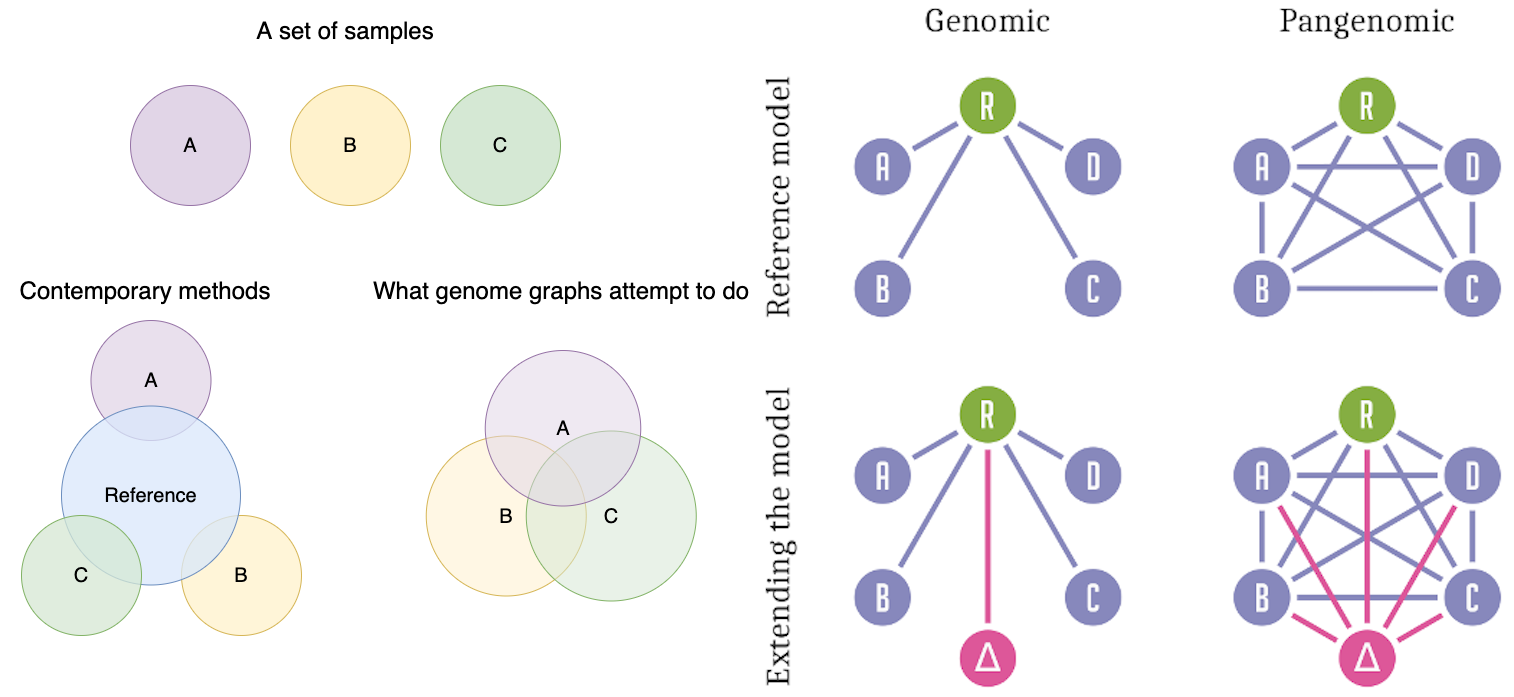
\includegraphics[width=0.75\textwidth]{../Figures/combined-all-vs-all.png}
\caption[All Against All Sample Comparison]{\label{fig:org00438a4}
Contemporary genomic methods compare each sample based on how it compares against a reference. A pangenomic method compares each sample against every other sample through the use of a reference pangenome graph. a) Shows this comparison using Venn diagrams and three samples A, B, and C. b) (from…)}
\end{figure}

The maximum likelihood phylogenetic tree in \ref{fig:org165769c} 
from \cite{githinjiAssessingUtilityMinority2018} showed that when using a linear 
reference of closely related samples such as those in a household outbreak it
was not possible to differentiate the samples with a level of certainty that was
satisfactory.

\begin{figure*}
\centering
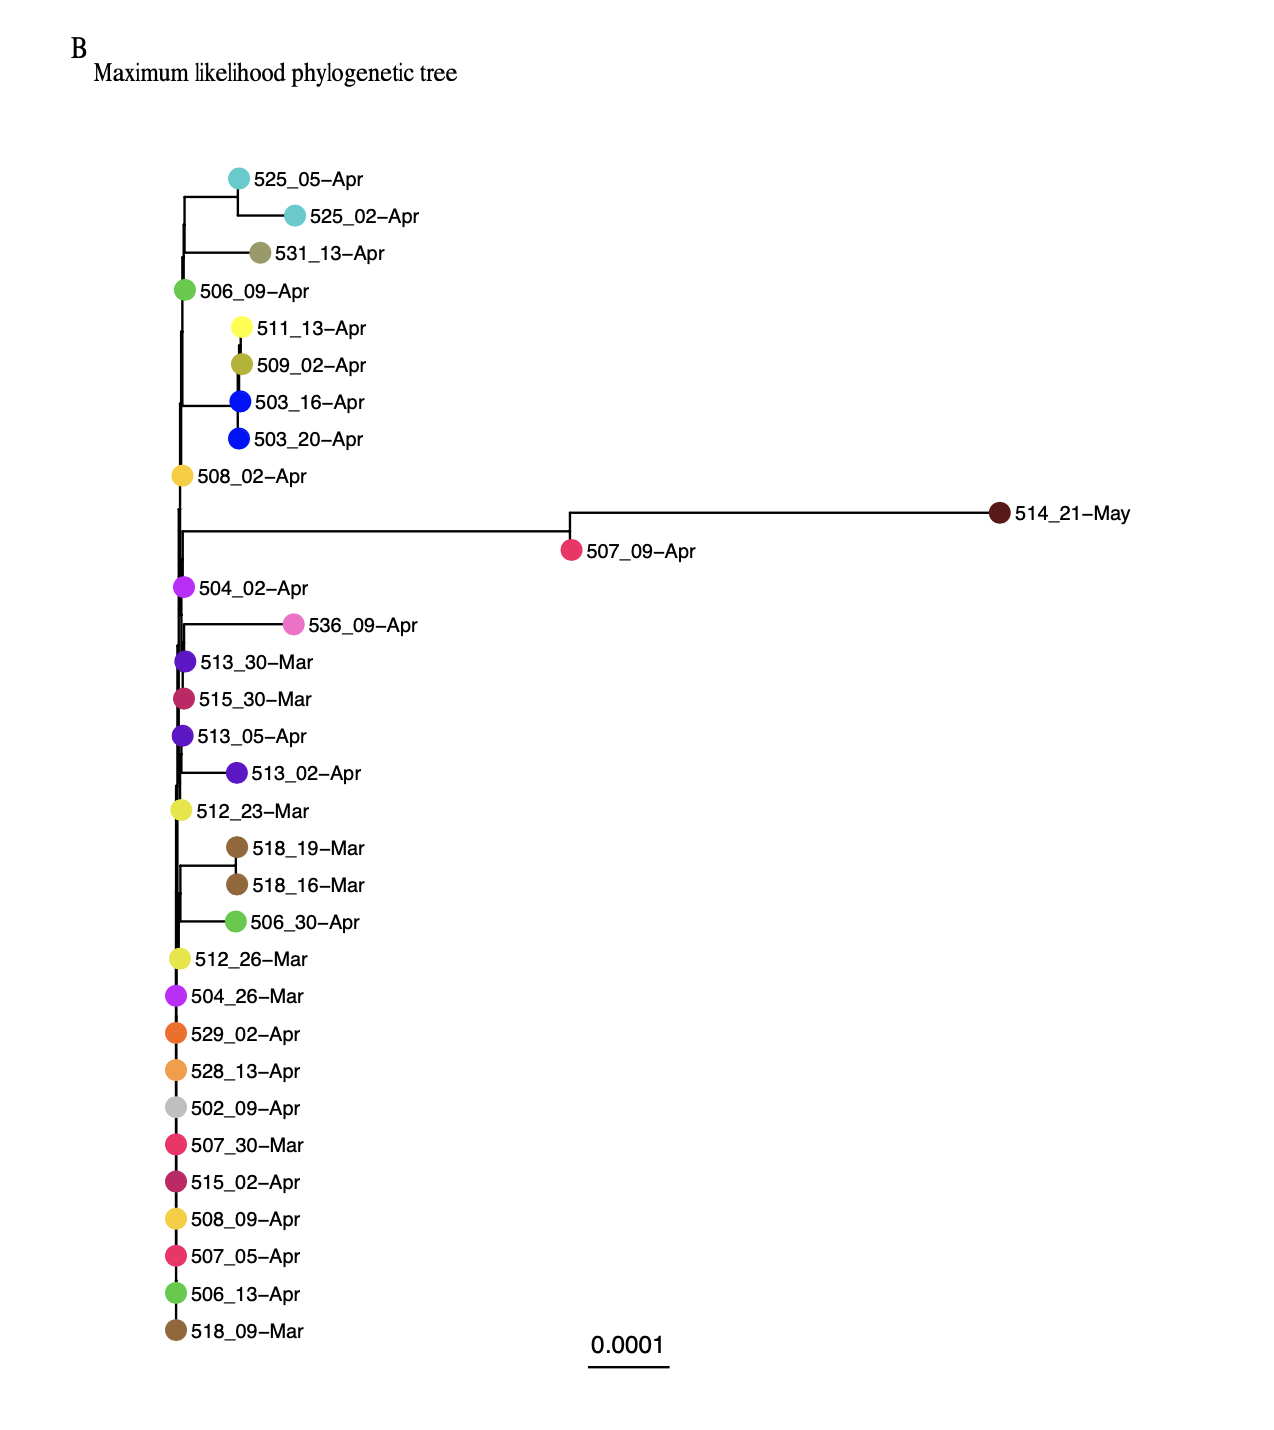
\includegraphics[width=0.7\textwidth]{../Figures/RSV/Githinji_HH20_ML_phylogenetic_tree.png}
\caption[RSV Maximum Likelihood Phylogenetic Tree]{\label{fig:org165769c}
The maximum likelihood phylogenetic tree of RSV from \cite{githinjiAssessingUtilityMinority2018}}
\end{figure*}

When using our method however, the coverage data seems to yield a somewhat 
linearly changing tree. This linearity is a factor of principal component analysis
which compares the distance of data from an origin but is also really good for
phylogenetics when assuming minimum evolution and one or few viral introductions 
then spread.

The branch lengths vary by a lot (as seen in the trees) but the topology stays 
the same depending on which of the principal components we used. 
The difference in branch length based on the first principal component 
expectedly maximizing the distance between them.
It seems that the first principal component is the one to use
when looking for visual cues of sample relatedness because it is the one that
most differentiates the samples and this is useful in getting a visual cue of
the relatedness.
The incorporation of the other four principal components is useful to get a 
more realistic view of the relatedness because they are also other measures of
differentiation and can be shown to give a more realistic view of the 
SARS-CoV-2 simulated reads for which we knew the sample relatedness going in.

\subsection{Strengths and limitations}
\label{sec:org7180502}
Genome graphs give insight into the genetic variation that was not as clear 
with previous tools. With their power we were able to analyze genomes at a
higher resolution and analyze their coverage. The method is simple and based 
on a concept that is easy to explain to people with little or no expertise in 
bioinformatics.

However, we note the method is not entirely conclusive and uses a naive
approach; it is an intuitionistic approach to compare samples facilitated by 
genome graphs which provide a higher resolution when looking at pangenomes or in
our case a virus quasispecies. We note that other machine learning techniques,
not only principal component analysis, could be used to analyze the coverage
data and models could be trained on an even larger dataset. It is possible and
actually favourable, because of the reduced computational cost, to have a world
where we look up new sample coverage against an already trained model instead 
of always running principal component analysis. 

\newpage
\section{Conclusion}
\label{sec:org934d6f8}
We provide a simple yet intuitionistic approach of comparing samples which
 facilitates an all versus comparison of samples without going through the 
reference as is the norm. This method involves using the depth of coverage under 
each node to  generate cladogram through neighbour joining. 
It provided a parsimonious tree that  correctly differentiated simulated
 SARS-CoV-2 reads and split a household RSV dataset to have two different
 introductions.

Future work will involve verifying that these trees are in fact differentiating these samples correctly and how it compares to contemporary methods of phylogenetics.

\newpage
\bibliographystyle{apacite}
\bibliography{../library}

\begin{appendices}
\subsection{Code}
\label{sec:org7ed2a8b}

\subsubsection{RSV}
\label{sec:org94c6f3a}
\paragraph{Quality Control and Adapter Trimming}
\label{sec:orgbcec5a3}
\begin{verbatim}
# concatenate the contents of all the files
# in ~/miniconda3/share/trimmomatic-0.39-1/adapters/ into one
# file, in my case adapters.fa and use those to trim adapters

trimmomatic PE \
 data/H_528_16_04/H_528_16_04_1.fastq.gz \
 data/H_528_16_04/H_528_16_04_2.fastq.gz \
 trimmed_forward_paired.fq.gz trimmed_forward_unpaired.fq.gz \
 trimmed_reverse_paired.fq.gz trimmed_reverse_unpaired.fq.gz \
 ILLUMINACLIP:adapters/adapters.fa:2:35:10:2:keepBothReads \
 SLIDINGWINDOW:4:35
\end{verbatim}

\paragraph{Concatenate Reads into Text File}
\label{sec:orgc725eae}
\begin{verbatim}
find $(pwd)/data -d -name '*interleave*fq' > sequences.txt
\end{verbatim}

\paragraph{Problematic RSV Sequences}
\label{sec:org1fd777a}
\begin{verbatim}
data/H_536_09_04/H_536_09_04_interleaved.fq:1271846:AGAACTCAGTGTAGGTAGAATGGTTGGCTGATCAATATCTCTAATGATTTTGGTCTGTGAATCAACTGTCATAAGAGAATTCTATCAAAGTTGAATTCCGAATCCTTGGGTCAATGACTGGGTGCACCCATTCTTCTAATGTGCTCTGTC
data/H_506_13_04/H_506_13_04_interleaved.fq:3831798:AGAACTCAGTGTAGGTAGAATGGTTGGCTGAGTAGGTAGATGGAGGCAGGTGCATGTGTGATGGGAAGTGTGGTGACGGGTTGTGTGGGCACACGGGATGAGGCGCAGATGGCTGGGGGTTTGGGAGGGGAATGGGTGGGAGAAGGAGGC
\end{verbatim}

\paragraph{Minia Fragment Assembly}
\label{sec:orge1e0d60}
\begin{verbatim}
minia -in ../sequence_paths.txt \
  -kmer-size 31 \
  -abundance-min 1000 \
  -nb-cores 8
\end{verbatim}

\paragraph{Graph Bluntification Using Stark}
\label{sec:org8869ee9}
\begin{verbatim}
stark -i input_file_name \
  -o stark_bluntify.gfa \
  -s cpu-consuming
\end{verbatim}

\paragraph{Odgi Graph Preparation}
\label{sec:orgfde9b87}
\begin{verbatim}
#!/usr/bin/env bash

# premap.sh

InputGFA=$1
BuildVG="build-odgi.vg"
ChoppedVG="chopped-odgi.vg"
SortedVG="sorted-odgi.vg"
ViewGFA="view-odgi.gfa"

echo "Using $InputGFA"
odgi build \
     -s \
     -g ${InputGFA} \
     -o ${BuildVG}

echo "Chopping to size 1024"
odgi chop \
     -i build-odgi.vg \
     -c 1024 \
     -o ${ChoppedVG}

echo "Sorting"
odgi sort \
     -i chopped-odgi.vg \
     -o ${SortedVG}

echo "Generating GFA $ViewGFA"
odgi view \
     -i sorted-odgi.vg \
     -g \
     > ${ViewGFA}

# Run with
./pre-map.sh stark_bluntify.gfa
\end{verbatim}

\paragraph{RSV VG View}
\label{sec:orgea2a9b4}
\begin{verbatim}
vg view -Fv view-odgi.gfa > graph.vg
\end{verbatim}

\paragraph{RSV VG Index}
\label{sec:org43d7006}
\begin{verbatim}
vg index -x graph.xg -g graph.gcsa graph.vg
\end{verbatim}

\paragraph{RSV VG Map Script}
\label{sec:org3e82afb}
\begin{verbatim}
#!/usr/bin/env bash

Graphname="graph"
# Using a gams dir to put the gam files
GAMDir="gams"

# For each file in the sequence list, call vg to map it to the graph
while read Filepath;
do
    # paramter expansion http://mywiki.wooledge.org/BashFAQ/073
    Filename=${Filepath##*/}
    FileStub=${Filename%_*}

    echo "Mapping $FileStub"
    vg map \
       -f ${Filepath} \
       -x ${Graphname}.xg \
       -g ${Graphname}.gcsa \
       > ${GAMDir}/${FileStub}.gam

# Run with
./map.sh < ../sequence_paths.txt
\end{verbatim}

\paragraph{Generate GAM}
\label{sec:org919e7ae}
\begin{verbatim}
vg view -a -k gams/H_513_02_04.gam > Images/H_513_02_04.gamp
vg view -K -j Images/H_513_02_04.gamp > Images/H_513_02_04_GAMP.json
cat Images/H_513_02_04_GAMP.json | jq | less
\end{verbatim}

\paragraph{VG Pack Script}
\label{sec:org5a35cf6}
\begin{verbatim}
#!/usr/bin/env bash

# Loop through each gam file
Graphname="graph"
CoverageDir="coverage"

while read Filepath;
do
    # parameter expansion http://mywiki.wooledge.org/BashFAQ/073
    FileStub=${Filepath%.*}

    vg pack \
       -d \
       -x ${Graphname}.xg \
       -g ${Filepath} \
       > ${CoverageDir}/${FileStub}.pack.table
done

# Run with

find $(pwd)/gams -d -name '*.gam' > gams.txt
./map.sh < gams.txt
# or
./coverage.sh < find $(pwd)/gams -d -name '*.gam'
\end{verbatim}



\subsubsection{SARS-COV-2}
\label{sec:org09a52b2}
\paragraph{Efetch}
\label{sec:orgc62dd48}
\begin{verbatim}
efetch -db=nuccore -format=fasta -id=NC_045512.2 > \
 ~/projects/Masters/verify/data/refs/COVID_19.fa
\end{verbatim}

\paragraph{dwgsim Read Simulation}
\label{sec:orge046742}
\begin{verbatim}
# Set ref as a var
export REF=~/projects/Masters/verify/data/refs/COVID_19.fa
dwgsim -N 1000 $REF covid_19_sim_1
dwgsim -N 1000 $REF covid_19_sim_2

# Increase the mutation rate from the default 0.0010 to 0.0100

dwgsim -N 1000 -r 0.0100 $REF covid_19_sim_3
\end{verbatim}

\paragraph{Bifrost Fragment Assembly}
\label{sec:org98bbb11}
\begin{verbatim}
Bifrost build \
  -c \
  -k 31 \
  -s sequences.txt \
  -o SARS-CoV-2
\end{verbatim}

\paragraph{Gimbricate Graph Bluntification}
\label{sec:org66af93d}
\begin{verbatim}
gimbricate -d  \
  -g SARS-CoV-2.gfa \
  -p SARS-CoV-2.paf \
  -f SARS-CoV-2.fasta \
  > SARS-CoV-2.gimbry.gfa

\end{verbatim}

\paragraph{Seqwish Graph Induction}
\label{sec:org4203a85}
\begin{verbatim}
seqwish \
  -s SARS-CoV-2.fasta \
  -p SARS-CoV-2.paf \
  -g SARS-CoV-2.seqwish.gfa
\end{verbatim}

\paragraph{Odgi Build}
\label{sec:orge429cca}
\begin{verbatim}
odgi build \
  -s \
  -g SARS-CoV-2.seqwish.gfa \
  -o SARS-CoV-2-odgi-graph.vg
\end{verbatim}

\paragraph{Odgi Chop}
\label{sec:org03bcda8}
\begin{verbatim}
odgi chop \
  -i SARS-CoV-2-odgi-graph.vg \
  -c 1024 \
  -o SARS-CoV-2-odgi-chopped.vg
\end{verbatim}

\paragraph{Odgi Sort}
\label{sec:org53404ea}
\begin{verbatim}
odgi sort \
 -i SARS-CoV-2-odgi-chopped.vg \
 -o SARS-CoV-2-odgi-sorted.vg
\end{verbatim}

\paragraph{Odgi View}
\label{sec:org1ac9d3b}
\begin{verbatim}
odgi view \
 -i SARS-CoV-2-odgi-sorted.vg \
 -g \
 > SARS-CoV-2-odgi.gfa
\end{verbatim}

\paragraph{SARS-CoV-2 VG View}
\label{sec:org9e75513}
\begin{verbatim}
# vg view help
Usage: vg view [options] [ <graph.vg> | <graph.json> | <aln.gam> | <read1.fq> [<read2.fq>] ]
options:
    -g, --gfa                  output GFA format (default)
    -F, --gfa-in               input GFA format, reducing overlaps if they occur
    -v, --vg                   output VG format

# Run vg view
vg view -Fv SARS-CoV-2-odgi.gfa > SARS-CoV-2-vg.vg

\end{verbatim}

\paragraph{SARS-CoV-2 VG Index}
\label{sec:org895f7dc}
\begin{verbatim}
# vg index help
xg options:
    -x, --xg-name FILE     use this file to store a succinct, queryable version of the graph(s), or read for GCSA indexing
gcsa options:
    -g, --gcsa-out FILE    output a GCSA2 index to the given file
    -k, --kmer-size N      index kmers of size N in the graph (default 16)

# Run vg index
vg index -x SARS-CoV-2.xg -g SARS-CoV-2.gcsa SARS-CoV-2-vg.vg
\end{verbatim}

\paragraph{SARS-CoV-2 VG Pack Script}
\label{sec:orgfeb089b}
\begin{verbatim}
# vg pack help
-d, --as-table         write table on stdout representing packs

# Run vg pack in a loop
for i in {1..3}
do 
 vg pack \
   -x SARS-CoV-2.xg \
   -g SARS-CoV-2-${i}.gam \
   -d \
   > SARS-CoV-2-${i}.pack.table
done
\end{verbatim}

\end{appendices}
\end{document}
